
\chapter{Sistemas de ecuaciones lineales: teorema de Rouché}	
\chaptermark{S.E.L.: th. Rouché}	\label{SEL}

	
\section{Rango de una matriz}\label{rangos}

\begin{defi}.



Se dice que una matriz $M\in \mathcal M_{m \times n}(\mathbb R)$ es una \colorbox{LightYellow}{\textbf{`matriz escalonada'}}:

\noindent  --- por filas, si:

\hspace{3mm} 1.	Todas las filas de $M$ (si las hay) cuyos elementos son todos nulos aparecen en la parte inferior de la matriz. 

\hspace{3mm} 2.	El primer número no nulo (comenzando por la izquierda) en cualquier fila no nula de $M$ recibe el nombre de pivote de esa fila. 

\hspace{3mm} 3.	Cada fila de $M$ (exceptuando, por lo general, a la primera) comienza con una sucesión de ceros, de manera que siempre contiene (al menos) un cero más que la fila anterior. En otras palabras, el pivote en cualquier fila está a la derecha del pivote de la fila anterior. 

\noindent  --- por columnas, si:

\hspace{3mm} 1.	Todas las columnas de $M$ (si las hay) cuyos elementos son todos nulos aparecen a la derecha de la matriz. 

\hspace{3mm} 2.	El primer número no nulo (comenzando por arriba) en cualquier columna no nula de $M$ recibe el nombre de pivote de esa fila. 

\hspace{3mm} 3.	Cada columna de $M$ (exceptuando, por lo general, a la primera) comienza con una sucesión de ceros, de manera que siempre contiene (al menos) un cero más que la columna anterior. En otras palabras, el pivote en cualquier columna está más abajo que el pivote de la fila anterior. 
\end{defi}


\begin{ejem}.

Son matrices escalonadas: $\left( \begin{matrix} 1&2&5\\0&1&1\\0&0&1  \end{matrix} \right); \qquad \left( \begin{matrix} 1&3&2&1\\0&1&7&8\\0&0&1&3\\0&0&0&3 \end{matrix} \right)$

No lo son: $\left( \begin{matrix} \colorbox{yellow}{0}&\colorbox{yellow}{0}&5\\ \colorbox{yellow}{0}&3&7\\ \colorbox{yellow}{0}&\colorbox{yellow}{0}&4  \end{matrix} \right); \qquad \left( \begin{matrix}  1&3&2&1\\\colorbox{yellow}{0}&4&7&8\\\colorbox{yellow}{0}&\colorbox{yellow}{0}&\colorbox{yellow}{0}&3\\ \colorbox{yellow}{0}&\colorbox{yellow}{0}&5&4  \end{matrix} \right)$
	
\end{ejem}

\begin{defi}.

\colorbox{LightYellow}{Se llama \textbf{`Rango'} de una matriz $M$, $\; rg(M)\;$, al número de filas}

 \colorbox{LightYellow}{(columnas) no-nulas que quedan en la matriz escalonada $M_e$.}

%\fcolorbox{frame color}{box background color}{...}	
\end{defi}

Este número, por filas o columnas, coincide y corresponde al `número de filas (columnas) \emph{Linealmente Independientes}' que tiene la matriz. Este importante concepto lo estudiaremos en el próximo capítulo de `Espacios Vectoriales'.

Para, dada una matriz $M_{m \times n}$, obtener su rango, $\; rg(M) \;$, veremos dos métodos:

\hspace{3mm} ----- El \textbf{método de Gauss} de la matriz escalonada.

\hspace{3mm} ----- El \textbf{método de los orlados} (por adjuntos).

%$\left( \begin{matrix}   \end{matrix} \right)$
\subsection{Rango por Gauss} \label{escalonado}


Para, a partir de una matriz cualquiera $M$ obtener una matriz escalonada $M_e$ se usan transformaciones elementales de Gauss en que se puede cambiar el orden tanto de filas como de columnas (estrategia del pivote). En la práctica, en vez de llevar las filas de ceros al final, las podemos tachar.

Observación: Generalmente, cuando se utilizan operaciones elementales se pueden obtener diferentes matrices escalonadas por filas equivalentes a la de partida. Es decir, no existe una única matriz escalonada por filas asociada a una matriz A. 
%$\left( \begin{matrix}   \end{matrix} \right)$

\begin{ejem}
Calcula el rango de  $M	= \left( \begin{matrix} 1&2&0&3&4\\0&0&0&2&3\\1&2&0&5&7\\0&0&0&0&1  \end{matrix} \right) \to M_e$

$Me \to [F3\to F3-F1] \to \left( \begin{matrix} 1&2&0&3&4\\0&0&0&2&3\\0&0&0&2&3\\0&0&0&0&1  \end{matrix} \right) \to [F3\to F3-F2]  \to   \left( \begin{matrix} 1&2&0&3&4\\0&0&0&2&3\\ \text{\textst{ 0 }}&\text{\textst{ 0 }}&\text{\textst{ 0 }}&\text{\textst{ 0 }}&\text{\textst{ 0 }} \\0&0&0&0&1  \end{matrix} \right) \; \Rightarrow \; \;  \boldsymbol{ rg(M)=3 }$ 
\end{ejem}


\underline{Observación}: muchos textos dicen que calcular un rango por Gauss consiste en triangularizar la matriz de modo que por debajo de la diagonal principal todos los elementos sean cero. Entonces, prescindiendo de las trivialidades (filas de cero), el número de filas que quedan es el rango de la matriz. Esto es FALSO, hay que llegar a una MATRIZ ESCALONADA, no solo TRIANGULAR. Véase el siguiente ejemplo:

\begin{ejem}

$\left| \begin{matrix}  1&2&0&3&4\\0&0&0&2&3\\0&0&0&2&3\\0&0&0&0&1 \end{matrix} \right| \Rightarrow rango \; 4$. Falso, esta matriz es triangular pero no está escalonada, la fila $3$ no tiene más ceros a la izquierda que la dos (si nos damos cuenta, es la misma y podemos prescindir de ella). Al seguir buscando ceros en $F3\to F3-F2$ obtenemos una trivialidad:

$\left| \begin{matrix}  1&2&0&3&4\\0&0&0&2&3\\ \text{\textst{ 0 }}&\text{\textst{ 0 }}&\text{\textst{ 0 }}&\text{\textst{ 0 }}&\text{\textst{ 0 }}  \\0&0&0&0&1 \end{matrix} \right| \Rightarrow rango \; 3$.

	
\end{ejem}


\subsection{Rango por adjuntos. Método de los orlados.}

\begin{defi}.

Si en una matriz de orden $m \times n$ tomamos $k$ filas y $k$ columnas y formamos  un determinante de orden $k$ se le llama menor de orden $k$, $\; M_k$.

Si a este $M_k$ se le añaden una fila y una columna cualesquiera de $M$ se obtiene un menor de orden $k+1$  que se llama \textbf{menor orlado}.

Definimos el rango de la matriz $M$ como   \colorbox{LightYellow}{$rg(M)=\; $el orden del mayor}  \colorbox{LightYellow}{ menor no-nulo} obtenido de $M$

Dada $M_{m \times n}$ siempre se verificará que  \colorbox{LightYellow}{$\boxed{ \; rg(M) \le min\{ m,\; n \} \; }$}. Para encontrar el rango de una matriz bastará con encontrar un $M_k \neq 0$ tal que todos los $M_{k+1}$ orlados a través de él sean cero. Para esto usaremos el:

\end{defi}

\textbf{Método de los Orlados}: partimos de un menor no nulo y vamos orlando con las filas y columnas restantes hasta encontrar el máximo menor no nulo de la matriz. Su orden es el rango. 

En la práctica:

----- Se prescinde de todas las líneas formadas por ceros, ya que al añadir filas o columnas de ceros a un determinante, éste resulta nulo.

----- Si a simple vista se descubre alguna línea que sea igual o proporcional a otras, se prescinde de ella.


\begin{ejem} Calcula el rango de  $M	= \left( \begin{matrix} 1&2&0&3&4\\0&0&0&2&3\\1&2&0&5&7\\0&0&0&0&1  \end{matrix} \right)$

Rápidamente encontramos en $M$ un menor de orden $2$ distinto de cero:



$M_2=\left| \begin{matrix} 3&4\\2&3  \end{matrix} \right|=9-8=1\neq 0$. Luego $rg(M)\ge 2$, veamos si puede ser $3$. Para ello vamos a `orlar' el menor anterior con filas y columnas para obtener menores de orden $3$ hasta que encontremos uno de ellos distinto de cero ($rg(M)\ge 3$) o comprobemos que todos ellos son cero ($rg(M)=2$). \textcolor{gris}{\emph{Obsérvese que a partir de nuestro menor de orden $2$ distinto de cero $(M_2$) podemos encontrar hasta $6$ menores de orden $3$, orlando con F3C3, F4C3, F3C2, F4C2, F3C1 y F4C1}}

Podemos orlar a $M_2$ con elementos de la $C3$, pero al ser todo ceros, seguro que el menor de orden $3$ que busquemos resulta nulo, así que empecemos orlando a $M_2$ con elementos de $C2$, podemos añadir la $F3$ o la $F4$, empecemos con $M_2,\; C3,\; F3$:

$\left| \begin{matrix} 2 & \boxed{3} & \boxed{4} \\ 0 & \boxed{2} & \boxed{3} \\ 2 & 5 & 7  \end{matrix} \right| = 28+0+18-(16+30+0)=46-46=0$

Veamos lo que ocurre al orlar con la $F4$, es decir:  $M_2,\; C3,\; F4$:

$M_3=\left| \begin{matrix} 2 & \boxed{3} & \boxed{4} \\ 0 & \boxed{2} & \boxed{3} \\ 0 & 0 & 1  \end{matrix} \right| = 2\; (-1)^{1+1}\cdot 1=2\neq 0 \Rightarrow  rg(M)\ge 3$

A partir ahora de este $M_3 \neq 0$, continuamos orlando. Ahora solo podemos añadir la $C1$ y $F3$ para obtener:

$\left| \begin{matrix} 1& \boxed{2} & \boxed{3} & \boxed{4} \\ 0 & \boxed{0} & \boxed{2} & \boxed{3} \\ 1 & 2 & 5 & 7 \\ 0 & \boxed{0} & \boxed{0} & \boxed{1}  \end{matrix} \right| = \; [C2=2\cdot C1] \; = 0 \Rightarrow rg(M) \neq 4$

Conclusión: el rango de $M$ es: $\quad \boldsymbol{rg(M)=3}$ 

\emph{\textcolor{gris}{En el próximo tema diremos que en $M$ hay $3$ filas independientes, $F1, F2, F4$ o $3$ columnas independientes $C2, C3, C4$. Podremos prescindir de $F3$, pues es `combinación lineal de las demás' o de la $C1$, por ser `combinación lineal' de  $C2, C3, C4$}}
	
\end{ejem}



Resumiendo:

\textbf{Cálculo del rango de una matriz $A$ mediante determinantes (orlando menores)}

1) Si la matriz es nula, su rango es $0$ y hemos terminado. En caso contrario, seguimos.

2) Buscamos un menor fácil de orden $2$ no nulo: $M$. Si esto no es posible, el $rg(A)=1$ y hemos terminado.

3) Elegimos una fila de $A$ que no esté en $M$ .Orlamos $M$ : completamos un nuevo menor con elementos de dicha fila y una columna que no esté en $M$. Si dicho menor vale $0$, elegimos otra columna, y así hasta completar todas las columnas de $A$, siempre con dicha fila.

\hspace{5mm} a) Si todos esos menores valen $0$, la fila elegida es `combinación lineal' de las filas que están en $M$, y puede ignorarse a efectos del cálculo del rango. En ese caso, repetimos el paso $2$ con otra fila, y así hasta completar todas las filas de $A$.

\hspace{5mm}  b) Si alguno de esos menores es no nulo, el rango de $A$ es el orden de dicho menor, como mínimo. Llamamos $M$ a dicho nuevo menor no nulo y repetimos el
paso $3$ con otra fila.

4) El rango de $A$ será el orden del máximo menor no nulo $M$ encontrado con este procedimiento. Las filas y columnas de $A$ que figuran en $M$ son `linealmente independientes'. A dicho menor $M$ se le llama \textbf{menor principal}. Las filas y columnas que no están en $M$ son `combinación lineal' de las que sí aparecen en $M$. (más en el próximo tema de espacios vectoriales).

\vspace{20mm}

\section{Método de Cramer}

\begin{defi}
Se dice que un SEL es de Cramer si tiene el mismo número de ecuaciones que de incógnitas y, escrito matricialmente, el determinante de la matriz de los coeficientes es distinto de cero.	
\end{defi}


Un sistema de ecuaciones lineales `cuadrado', es decir, con tantas ecuaciones como incógnitas, se puede interpretar como una ecuación matricial:

$\begin{cases} a_{11}x_1+a_{12}x_2 + \cdots + a_{1n}x_n &=b_1 \\
a_{12}x_1+a_{22}x_2 + \cdots + a_{2n}x_n &=b_2 \\
\cdots + \cdots + \cdots + \cdots + \cdots  &=\cdots \\
a_{n1}x_1+a_{n2}x_2+\cdots +a_{nn}x_n &=b_n  \end{cases} \quad \Leftrightarrow \quad \boxed{\; AX=B\; \; }$	,

donde:
$A=\left( \begin{matrix}  a_{11}&a_{12}& \cdots &a_{1n} \\
a_{12} &a_{22} &\cdots &a_{2n} \\
\cdots & \cdots & \cdots & \cdots  \\
a_{n1} &a_{n2} &\cdots &a_{nn}    \end{matrix} \right); \; X=\left( \begin{matrix} x_1\\x_2\\ \vdots \\x_n \end{matrix} \right); \; B=\left( \begin{matrix} b_1\\b_2\\ \vdots \\b_n \end{matrix} \right)$

$A$ es la matriz de los coeficientes, $X$ la de incógnitas y $B$ la de términos independientes.

El que este \colorbox{LightYellow}{SEL-cuadrado} sea de \colorbox{LightYellow}{Cramer} implica que \colorbox{LightYellow}{$\boldsymbol{ \; |A|\neq 0\; }$} $\; \to \exists A^{-1} \to \boldsymbol{ X=A^{-1}B }$

Recordando que la matriz adjunta de $A$ está formada por los elemento $A_{ij}$ y que la inversa es uno partido por el determinante de la matriz adjunta de la matriz \emph{traspuesta}, esta ecuación se puede escribir como:

\vspace{3mm}

\centerline{$\left( \begin{matrix} x_1\\x_2\\ \vdots \\ \boldsymbol{ x_i} \\ \vdots \\x_n  \end{matrix} \right) =
\dfrac 1 {|A|}\;
\left( \begin{matrix} A_{11}&A_{21}& \cdots &A_{n1}\\
A_{12}&A_{22}& \cdots & A_{n2}\\
\vdots & \vdots & \ddots & \vdots \\
\boldsymbol{A_{1i}}&\boldsymbol{A_{2i}}& \cdots & \boldsymbol{A_{ni}} \\
\vdots & \vdots & \ddots & \vdots \\
A_{1n}&A_{2n}& \cdots & A_{nn}  \end{matrix} \right) 
\cdot \boldsymbol{\left( \begin{matrix} b_1\\b_2\\ \vdots \\ b_i \\ \vdots \\ b_n  \end{matrix} \right)}$}

\justify 

\vspace{2mm}
\centerline{$x_i=\dfrac 1 {|A|}\; \left( b_1A_{1i}+b_2A_{2i}+\cdots +b_nA_{ni}  \right) = \to $}

\vspace{2mm}
que es el desarrollo del determinante de la matriz $A$ en que se ha sustituido la columna-$i$ de coeficientes por la de términos independientes ($b_i$) y se ha desarrollado por adjuntos de Laplace de la columna-$i$:

\vspace{2mm}
\centerline{$\to = \dfrac 1 {|A|}\; \left| \begin{matrix} 
a_{11}& a_{12}& \cdots & \textcolor{red}{b_1} & \cdots & a_{1n} \\
a_{21}& a_{22}& \cdots & \textcolor{red}{b_2} & \cdots & a_{2n} \\
\vdots & \vdots & \ddots & \vdots & \ddots & \vdots \\
a_{n1}& a_{n2}& \cdots & \textcolor{red}{b_n} & \cdots & a_{nn} \\
 \end{matrix} \right| $}
 
 Luego, resolver un sistema de Cramer (cuadrado con $|A|\neq 0$) consiste en calcular $(n+1)$ determinantes, uno para cada incógnita más el de los coeficientes y el resultado de cualquier incógnita consiste en calcular el determinante de $A$ en que se ha sustituido la columna correspondiente a la incógnita a calcular por la columna de términos independientes y dividirlo por el determinante de $A$.
 
\noindent Cramer $\begin{cases} n \times n \\ |A|\neq 0 \end{cases} \Rightarrow \;$ \colorbox{LightYellow}{$  \boxed{\; \textcolor{red}{x_i}= \dfrac 1 {|A|}\; \left| \begin{matrix} 
a_{11}& a_{12}& \cdots & \textcolor{red}{b_1} & \cdots & a_{1n} \\
a_{21}& a_{22}& \cdots & \textcolor{red}{b_2} & \cdots & a_{2n} \\
\vdots & \vdots & \ddots & \vdots & \ddots & \vdots \\
a_{n1}& a_{n2}& \cdots & \textcolor{red}{b_n} & \cdots & a_{nn} \\
 \end{matrix} \right|\;}$}
 
 \begin{ejem}
 Resuelve por Cramer, si es posible: $\begin{cases}
x+2y-z&=-3\\x\quad \quad +\; z&=1\\2x-y+2z&=4	
\end{cases}$

Tenemos un sistema cuadrado: 3 ecuaciones con 3 incógnitas, con $|A|=\left| \begin{matrix} 1&2&-1\\1&0&1\\2&-1&2   \end{matrix} \right| = 0+1+4-(0-1+4)=5-3= \textcolor{blue}{\boldsymbol{2}} \neq 0 \to \;$ sí es resoluble por Cramer:

$\boldsymbol{x}=\dfrac 1 {\textcolor{blue}{\boldsymbol{2}}} \; \left| \begin{matrix} \textcolor{red}{3}&2&-1\\ \textcolor{red}{-1}&0&1\\ \textcolor{red}{4}&-1&2   \end{matrix} \right| = \dfrac 1 4 \; [0+1+8 -(0-3+4 )] \dfrac 1 2 (9-7)=\boldsymbol{1}  $

$\boldsymbol{y}=\dfrac 1 {\textcolor{blue}{\boldsymbol{2}}} \; \left| \begin{matrix} 1&\textcolor{red}{3}&-1\\1&\textcolor{red}{-1}&1\\2&\textcolor{red}{4}&2   \end{matrix} \right| = \dfrac 1 4 \;[2-4-6 -(-2+4-6 )]=\dfrac 1 2 [-8-(-4)]  = \boldsymbol{2} $

$\boldsymbol{z}=\dfrac 1 {\textcolor{blue}{\boldsymbol{2}}} \; \left| \begin{matrix} 1&2&\textcolor{red}{3}\\1&0&\textcolor{red}{-1}\\2&-1&\textcolor{red}{4}   \end{matrix} \right| = \dfrac 1 4 \;[0+3+4 -(0-1+8 )] =\dfrac 1 2 (7-7)  =\boldsymbol{ 0} $

SCD

 \end{ejem}

\emph{Ventajas e inconvenientes} del método de Cramer frente al método de Gauss:

\begin{itemize}
\item Si el sistema es de Cramer (que no lo son todos los SEL), Cramer nos permite, sin resolver todo el sistema, conocer el valor de cualquier incógnita del sistema sin más que calcular un cociente de determinantes.

\item Pero el SEL puede no ser de Cramer y Gauss es válido para cualquier tipo de SEL.
\end{itemize}


%$\left| \begin{matrix}   \end{matrix} \right|$
%$\left( \begin{matrix}   \end{matrix} \right)$

%$\left( \begin{matrix}   \end{matrix} \right)$
\section{Teorema de Rouché-Frobenius}


Consideremos un SEL cualquiera, de $m$ ecuaciones lineales con $n$ incógnitas:

\centerline {$\begin{cases} a_{11}x_1+a_{12}x_2 + \cdots + a_{1n}x_n &=b_1 \\
a_{12}x_1+a_{22}x_2 + \cdots + a_{2n}x_n &=b_2 \\
\cdots  \cdots  \cdots  \cdots  \cdots  \cdots \cdots  \cdots  \cdots  &= \cdots \\
a_{m1}x_1+a_{m2}x_2+\cdots +a_{mn}x_n &=b_m  \end{cases} $	,}

\justify
Llamamos matrices $A$ de los coeficientes y $A^*$ matriz ampliada a las matrices:



$A=\left( \begin{matrix}  a_{11}&a_{12}& \cdots &a_{1n} \\
a_{12} &a_{22} &\cdots &a_{2n} \\
\cdots & \cdots & \cdots & \cdots  \\
a_{m1} &a_{m2} &\cdots &a_{mn}    \end{matrix} \right); \; \; A^*=
\left( \begin{matrix}  a_{11}&a_{12}& \cdots &a_{1n} \\
a_{12} &a_{22} &\cdots &a_{2n} \\
\cdots & \cdots & \cdots & \cdots  \\
a_{m1} &a_{m2} &\cdots &a_{mn}    \end{matrix} \right|
\left. \begin{matrix} b_1\\b_2\\ \vdots \\ b_m \end{matrix} \right)$

Escrito en una sola matriz, por delante, hasta la barra vertical, tenemos a la matriz $A$, por detrás, sin la barra, la matriz $A^*$.

\begin{myblock}{Matriz de coeficientes y ampliada}

\centerline{$\; A=
\left( \begin{matrix}  a_{11}&a_{12}& \cdots &a_{1n} \\
a_{12} &a_{22} &\cdots &a_{2n} \\
\cdots & \cdots & \cdots & \cdots  \\
a_{m1} &a_{m2} &\cdots &a_{mn}    \end{matrix} \right|
\left. \begin{matrix} b_1\\b_2\\ \vdots \\ b_m \end{matrix} \right) \leftarrow A^*\; $}
\end{myblock}

\begin{teor}{Teorema de Rouché-Frobenius} \textcolor{gris}{(sin demostración)}

\vspace{4mm}

\centerline{\colorbox{LightYellow}{Un SEL es COMPATIBLE si $\boxed{\; rg(A)=rg(A^*)\; }$}}

\vspace{2mm}

-----  \colorbox{LightYellow}{si $\; rg(A)=rg(A^*) =$ número de incógnitas $\longrightarrow$ \textbf{SCD}}

-----  \colorbox{LightYellow}{si $\; rg(A)=rg(A^*) <$ número de incógnitas $\longrightarrow $ \textbf{SCI}}

----- \colorbox{LightYellow}{Obviamente, si $\; rg(A) \neq rg(A^*)$ $\longrightarrow $ \textbf{SI}}

En el caso $\; rg(A)=rg(A^*) <$ número de incógnitas , se llaman \textbf{ecuaciones principales del sistema} a las que forman el menor que dicta en rango, las otras ecuaciones se pueden eliminar y se llaman \textbf{incógnitas principales del sistema} a las que forman el menor que dicta el rango, las restantes se parametrizan, es decir, se les asignan valores reales cualesquiera, parámetros (letras griegas) y se pasan al segundo miembro quedando ahora un SEL cuadrado con determinante de los coeficientes principales distinto de cero con lo que el problema se puede resolver por Cramer (o por Gauss).
	
\end{teor}

\subsection{Aplicación a sistemas homogéneos}

Todo SEL de $m$ ecuaciones con $n$ incógnitas homogéneo ($b_1=b_2= \cdots = b_m=0$) admite siempre la  \textbf{solución trivial} $x_1=x_2= \cdots = x_n=0$, por lo que son siempre COMPATIBLES. 

Esto es evidente a la luz del teorema de Rouché puesto que si $A$ tiene rango $k$, $A^*$ también tendrá rango $k$ ya que $A^*$ no consiste más que en añadir a $A$ una columna de ceros y, obviamente, no altera el rango.

Según el teorema de Rouché, 

\hspace{2mm} ----- si $k=rg(A)=n=$número de incógnitas $\to $ el SEL es SCD, solución única: `la trivial' $(0,0, \cdots , 0)$

\hspace{2mm} -----  si $k=rg(A)<n=$número de incógnitas $\to $ el SEL es SCI,  infinitas soluciones (habrá que parametrizar) , entre ellas estará `la trivial' $(0,0, \cdots , 0)$


\section{Discusión de sistemas}

En ocasiones se nos presentará resolver SEL dependientes de uno o varios parámetros. Para ello usaremos el teorema de Rouché para determinar los rangos de $A$ y $A^*$ analizando todos los posibles casos que puedan presentarse en función del valor que tomen los parámetros del sistema (esto es lo que se llama `discusión de SEL') y resolviendo en los casos de compatibilidad.

\underline{Observación importante:} Para analizar el rango de una matriz usaremos el método ascendente de los orlados ---a no ser que nos pidan usar el método de Gauss--- (ver si la matriz tiene rango $1$; si lo tiene, ver si puede tener rango $2$; si es así, ver si el rango es $3$; etc). Pero si la matriz $A$ o $A^*$ son cuadradas procederemos al revés, viendo si pueden tener rango máximo, estudiaremos su determinante.

En el siguiente apartado de ejercicios resueltos veremos muchos ejemplos de discusión y resolución de SEL con el teorema de Rouché.
%$\text{\textst{ 0 }}$

% \text{\textst{ 0 }}&\text{\textst{ 0 }}&\text{\textst{ 0 }}&\text{\textst{ 0 }}&\text{\textst{ 0 }}

\section{Eliminación de parámetros $\divideontimes$}

\justify

\emph{La \textbf{eliminación de parámetros} es el proceso inverso a resolver un sistema de ecuaciones que sea compatible
indeterminado} (los sistemas que tienen infinitas soluciones  que  dependen  de uno o más parámetros), es decir,  pasar de las soluciones paramétricas de un SCI a las ecuaciones normales (implícitas, sin parámetros) que da lugar a esta solución. Así pues, lo que haremos es, dada la solución con parámetros encontrar el sistema de ecuaciones (o uno equivalente) que da lugar a esa solución.

En general, las soluciones de un sistema de ecuaciones expresadas en parámetros es (solución de un SEL que sea SCI):

\begin{equation*}
	\begin{cases}
	x_1=k_1+c_{11}t_1+c_{12}t_2+\cdots +c_{1p}t_p \\
	x_2=k_2+c_{21}t_1+c_{22}t_2+\cdots +c_{2p}t_p \\
	\cdots  \cdots \cdots \cdots \cdots \cdots \cdots \cdots \cdots \cdots \cdots\\
	x_n=k_n+c_{n1}t_1+c_{n2}t_2+ \cdots + c_{np}t_p
	\end{cases}
\end{equation*} 

\noindent que son las $n$-soluciones de las $n$-incógnitas dependientes de $p$-parámetros obtenidas del SEL de $m$-ecuaciones con $n$-incógnitas. Se trata de encontrar ese SEL, o uno equivalente, que proporcione esta misma solución.

\underline{Procedimiento para la eliminación de parámetros}:

1. Reescribir el sistema considerando los parámetros como incógnitas y las incógnitas como términos independientes:

\begin{equation*}
	\begin{cases}
	c_{11}t_1+c_{12}t_2+\cdots +c_{1p}t_p=x_1-k_1 \\
	c_{21}t_1+c_{22}t_2+\cdots +c_{2p}t_p=x_2-k_2 \\
	\cdots  \cdots \cdots \cdots \cdots \cdots \cdots \cdots \cdots \cdots \cdots\\
	c_{n1}t_1+c_{n2}t_2+ \cdots + c_{np}t_p=x_n-k_n
	\end{cases}
\end{equation*}

2. Este nuevo sistema ha de ser, también, \emph{\textbf{compatible}}, luego: 

\vspace{2mm}
\centerline{\colorbox{LightYellow}{$\; rg(A)=rg(A^*) \;$},} 

\noindent siendo $A$ y $A^*$ las  matrices de coeficientes y asociada a este nuevo sistema. Al exigir que se cumpla esta condición aparecen las relaciones entre las incógnitas que darán lugar al SEL buscado.

3. El número de ecuaciones obtenidas corresponde con el número de condiciones que debe haber entre las incógnitas $x_1,x_2,\cdots ,x_n$ (\textcolor{gris}{\emph{ligaduras}}) para que el sistema tenga solución. Se cumplirá que: (n=número de incógnitas)

\begin{equation*}
\colorbox{LightYellow}{\boxed{\text{ Número de ecuaciones } = n-rg(A)\; }}	
\end{equation*}

En en apartado `ejercicios resueltos' veremos ejemplos de resolución de eliminación de parámetros.


\section{Ejercicios}

\subsection{Ejercicios resueltos}

\begin{ejre} Estudia el rango de las siguientes matrices por el método de Gauss y por el método de los orlados.

$A=\left( \begin{matrix} 1&3&-2\\5&1&2  \end{matrix} \right); \quad
B=\left( \begin{matrix} -1&2&1\\2&11&5\\2&-1&3  \end{matrix} \right); \quad
C=\left( \begin{matrix}  1&2&-1&3\\3&7&0&11\\-4&-6&10&-3 \end{matrix} \right)$

$D=\left( \begin{matrix} 3&10&-1 \\ 1&3&-1 \\ -1&-1&8\\2&10&7  \end{matrix} \right); \quad 
E=\left( \begin{matrix} 2&-1&0&0\\0&0&2&-1\\0&2&-1&0\\2&0&-1&0  \end{matrix} \right)$
\end{ejre}
\begin{proofw}\renewcommand{\qedsymbol}{$\diamond$}

%\rule{45mm}{0.2pt}

------ \underline{Método de Gauss}
	
\noindent  * rango de $A \to   \left( \begin{matrix} 1&3&-2\\5&1&2  \end{matrix} \right) \to  [F2\to F2-5F1 \to \left( \begin{matrix} 1&3&-2\\0&-14&12  \end{matrix} \right) \Rightarrow \boldsymbol{rg(A)=2}$

\noindent  * rango de $B \to \left( \begin{matrix} -1&2&1\\2&11&5\\2&-1&3  \end{matrix} \right)  \to \left[ \begin{matrix}  F2\to F2+2F1 \\ F3\to F3+2F1 \end{matrix} \right] \to \left( \begin{matrix} -1&2&1\\0&15&7\\0&3&5  \end{matrix} \right)  \to [F3 \to 5F3-F2] \to \left( \begin{matrix} -1&2&1\\0&15&7\\0&0&18  \end{matrix} \right) \Rightarrow \boldsymbol{rg(B)=3}$

\noindent  * rango de $C \to \left( \begin{matrix}  1&2&-1&3\\3&7&0&11\\-4&-6&10&-3 \end{matrix} \right) \to   [C3 \leftrightarrow C1 ] \to \left( \begin{matrix}  -1&2&1&3\\0&7&3&11\\10&-6&4&-3 \end{matrix} \right) \to [F3 \to F3+10F1]\to \left( \begin{matrix}  -1&2&1&3\\0&7&3&11\\0&14&14&27 \end{matrix} \right) \to [F3 \to F3-2F2] \to \left( \begin{matrix}  -1&2&1&3\\0&7&3&11\\0&0&8&5 \end{matrix} \right) \Rightarrow \boldsymbol{rg(C)=3}$

\noindent  * rango de $D \to  \left( \begin{matrix} 3&10&-1 \\ 1&3&-1 \\ -1&-1&8\\2&10&7  \end{matrix} \right) [F1 \leftrightarrow F2 ] \to  \left( \begin{matrix} 1&3&-1 \\ 3&10&-1 \\  -1&-1&8\\2&10&7  \end{matrix} \right) \to \begin{cases} F2\to F2-3F1 \\ F3\to F3+F1  \\ F4\to  F4-2F1\end{cases} \to   \quad 
\left( \begin{matrix} 1&3&-1 \\ 0&1&2 \\  0&2&7\\0&4&9  \end{matrix} \right) \to \quad \begin{cases} F3\to F3-2F2 \\ F4 \to F4-4F2  \end{cases} \to 
\left( \begin{matrix} 1&3&-1 \\ 0&1&2 \\  0&0&3\\0&0&1  \end{matrix} \right) \to [F4\to 3F4-F3] \to  \left( \begin{matrix} 1&3&-1 \\ 0&1&2 \\  0&0&3\\ \text{\textst{ 0 }}&\text{\textst{ 0 }}&\text{\textst{ 0 }} \end{matrix} \right) \Rightarrow \boldsymbol{rg(D)=3}$


\noindent  * rango de $E \to \quad \left( \begin{matrix} 2&-1&0&0\\0&0&2&-1\\0&2&-1&0\\2&0&-1&0  \end{matrix} \right) \quad \to \quad   [F4 \to F4-F1] \quad \to \quad \left( \begin{matrix} 2&-1&0&0\\0&0&2&-1\\0&2&-1&0\\0&1&-1&0  \end{matrix} \right)  \to [F2 \leftrightarrow F4  ] \to \left( \begin{matrix} 2&-1&0&0\\0&1&-1&0\\0&2&-1&0\\0&0&2&-1  \end{matrix} \right) \to [F3 \to F3-2F2] \to \left( \begin{matrix} 2&-1&0&0\\0&1&-1&0\\0&0&1&0\\0&0&2&-1  \end{matrix} \right) \to [F4 \leftrightarrow F3 ] \to \left( \begin{matrix} 2&-1&0&0\\0&1&-1&0\\0&0&2&-1\\0&0&1&0  \end{matrix} \right) \to [F4 \to 2F4-F3] \to \left( \begin{matrix} 2&-1&0&0\\0&1&-1&0\\0&0&2&-1\\0&0&0&1  \end{matrix} \right) \to \Rightarrow \boldsymbol{rg(E)=4}$

\vspace{4mm}
------ \underline{Método de los orlados}

\noindent  * rango de $A \to   \left( \begin{matrix} \boxed{1}&\boxed{3}&-2\\\boxed{5}&\boxed{1}&2  \end{matrix} \right) \to \left( \begin{matrix} 1&3\\5&1  \end{matrix} \right)=1-15=-14\neq 0 \Rightarrow rg(A)\ge 2\;$ Como en $A$ hay una columna más pero no hay más filas, el rango no puede ser $3$, por lo que $\boldsymbol{ rg(A)=2}$


\noindent  * rango de $B \to \left( \begin{matrix} -1&2&1\\2&11&5\\2&-1&3  \end{matrix} \right)$; $B$ es cuadrada y nos preguntamos si tendrá rango máximo $3 \to \left| \begin{matrix} -1&2&1\\2&11&5\\2&-1&3  \end{matrix} \right|=-33-2+20-(22+5+12)=-15-39=-54\neq 0 \Rightarrow \boldsymbol{rg(B)=3}$


\noindent  * rango de $C \to \left( \begin{matrix}  \boxed{1}&\boxed{2}&-1&3\\\boxed{3}&\boxed{7}&0&11\\-4&-6&10&-3 \end{matrix} \right) \to $
$\left| \begin{matrix} 1&2\\3&7 \end{matrix} \right|=7-6=1\neq 0 \to rg(C)\ge 2\;$ 
Veamos si puede ser tres, a partir del $M_2$ marcado con cuadros en $C$, podemos orlar con $C2 y F3$ y con $C3 y F3$ a ver si encontramos un $M_3 \neq 0$ que asegure que el rango es $3$, en caso contrario (ambos determinantes fuesen cero), el rango de C se quedaría en $2$.

\noindent $\left| \begin{matrix} \boxed{1}&\boxed{2}&-1\\ \boxed{3}&\boxed{7}&0 \\-4&-6&10 \end{matrix} \right|=70+18+0-(28+0+60)=0$

\noindent $\left| \begin{matrix} \boxed{1}&\boxed{2}&3\\ \boxed{3}&\boxed{7}&11 \\-4&-6&-3 \end{matrix} \right|= -21-54-88-(-84-66-18)=5\neq 0 \Rightarrow \boldsymbol{rg(C)=3}$

\noindent \textcolor{gris}{\small{Luego en C hay $3$ fila o $3$ columnas independientes: $C \to \left( \begin{matrix}  \boxed{1}&\boxed{2}&-1&\boxed{3}\\\boxed{3}&\boxed{7}&0&\boxed{11}\\-4&-6&10&\boxed{-3} \end{matrix} \right)$}\normalsize{.}}

\noindent  * rango de $D \to  \left( \begin{matrix} \boxed{3}&\boxed{10}&-1 \\ \boxed{1}&\boxed{3}&-1 \\ -1&-1&8\\2&10&7  \end{matrix} \right) \to \left| \begin{matrix} 3&10\\1&3 \end{matrix} \right|=9-10=-1\neq 0 rg(D)\ge 2$. Podemos orlar con $C3 y F3$ o con $C3 y F4$ para ver si encontramos un $M_3 \neq 0$ que asegurase que el rango es $3$ (ya que $4$ no puede ser) o, si ambos determinantes son nulos, el rango de $E$ se quedaría en $2$.

\noindent $\left| \begin{matrix} \boxed{3}&\boxed{10}&-1\\\boxed{1}&\boxed{3}&-1\\ -1&-1&8 \end{matrix} \right|= 72+1+10-(3+3+80)=83-86=-3 \neq 0 \Rightarrow \boldsymbol{rg(D)=3}$ \textcolor{gris}{(estas tres filas o tres columnas son las linealmente independientes de $D$.)}

\noindent $\left| \begin{matrix} \boxed{3}&\boxed{10}&-1\\\boxed{1}&\boxed{3}&-1\\ 2&10&7 \end{matrix} \right|= \cdots$ Es innecesario seguir calculando. \textcolor{gris}{Tampoco es necesario escribir todos los posibles orlados, basta con encontrar uno distinto de cero o, eso sí, comprobar que todos sean cero. Lo hemos hecho así, y también en el caso siguiente, por motivos meramente didácticos.}



\noindent  * rango de $E \to \quad \left( \begin{matrix} 2&\boxed{-1}&\boxed{0}&0\\0&\boxed{0}&\boxed{2}&-1\\0&2&-1&0\\2&0&-1&0  \end{matrix} \right)  \to \left| \begin{matrix} -1&0\\0&2 \end{matrix} \right|=-2-0=-2\neq 0 \to rg(E)\ge 2$ Para comprobar si el rango es tres podemos orlar este $M_2$ con filas y columnas: $C1F3; \; C1F4; \; C4F3; \; C4F4$. Hay que ir calculando determinantes hasta encontrar uno distinto de cero ($rg(E)\ge 3$) o comprobar que todos ellos son cero ($rg(E)=2$). Vamos a por ellos:

\noindent $\left| \begin{matrix} 2&\boxed{-1}&\boxed{0}\\0&\boxed{0}&\boxed{2}\\0&2&-1 \end{matrix} \right| = 2(-1)^{1+1}\; (-2+0)=-4\neq 0 \to rg(E)\ge 3$

\noindent $\left| \begin{matrix} 2&\boxed{-1}&\boxed{0}\\0&\boxed{0}&\boxed{2}\\2&0&-1 \end{matrix} \right| = $ No es necesario continuar.

\noindent $\left| \begin{matrix} \boxed{-1}&\boxed{0}&0\\ \boxed{0}&\boxed{2}&-1 \\2&-1&0 \end{matrix} \right| = $ No es necesario continuar.

\noindent $\left| \begin{matrix} \boxed{-1}&\boxed{0}&0\\ \boxed{0}&\boxed{2}&-1\\0&-1&0 \end{matrix} \right| = $ No es necesario continuar.

\noindent A parir del $M_3\neq 0$ obtenido anteriormente podemos orlar con $C4F4$:

\noindent $(*)\; \left| \begin{matrix} 2&-1&0&0\\0&0&2&-1\\0&2&-1&0\\2&0&-1&0  \end{matrix} \right| = \quad [F4\to F4-F1]\quad = \left( \begin{matrix} 2&-1&0&0\\0&0&2&-1\\0&2&-1&0\\0&1&-1&0  \end{matrix} \right)\quad = \quad 2 (-1)^{1+1} \; \left| \begin{matrix} 0&2&-1\\2&-1&0\\ 1&-1&0 \end{matrix} \right|= 2 [0-2+0-(1+0+0)]=2\cdot(-3)=-6\neq 0 \Rightarrow \boldsymbol{rg(E)=4}$

Si recuerda el/la lector/a, dijimos anteriormente que si la matriz era cuadrada convenía hacer el estudio de los rangos al revés, viendo si el rango era máximo, con lo que hubiésemos empezado calculando $|E|=)*)=-6\neq 0 \Rightarrow \boldsymbol{rg(E)=4}$ y hubiésemos acabado antes. Quede este ejercicio como recuerdo de que en matrices cuadradas conviene hacer el estudio de los rangos de modo `descendente', empezando por ver si el rango es máximo.

\end{proofw}


\begin{ejre}
	Halla el rango de las siguientes matrices en función del valor que tome el parámetro:

\noindent $A=\left( \begin{matrix} 2&-1&-3&5\\2&2&-1&\lambda\\1&1&1&6\\3&1&-4&\lambda \end{matrix} \right); \;\;   \qquad 
B=\left( \begin{matrix} 1&k\\k&9\\2&6  \end{matrix} \right); \;\;   \qquad 
C=\left( \begin{matrix} 1&1&1&k\\k&k^2&1&1\\1&1&k&1  \end{matrix} \right);$

\noindent $D=\left( \begin{matrix} 1&1&2\\-1&a&-3\\1&a+2&1\\2&0&5  \end{matrix} \right); \;  \qquad 
E=\left( \begin{matrix} m-1&1&m&1\\1&m-1&m&1\\1&1&2&m-1  \end{matrix} \right)$
\end{ejre}

\begin{proofw}\renewcommand{\qedsymbol}{$\diamond$}


------ $rg(A)\; $: Como $A$ es cuadrada $(A_4)$, veamos si tiene rango máximo ($4$):

$\left| \begin{matrix} 2&-1&-3&5\\2&2&-1&\lambda\\ \boldsymbol{1}&\boldsymbol{1}&\boldsymbol{1}&\boldsymbol{6}\\3&1&-4&\lambda \end{matrix} \right|= \to \begin{cases} C2\to C2-C1 \\ C3\to C3-C1 \\ C4\to C4-6C1   \end{cases} \to = \left| \begin{matrix} 2&-3&-5&-7\\2&0&-3&\lambda-12\\ \boldsymbol{1}&\boldsymbol{0}&\boldsymbol{0}&\boldsymbol{0}\\3&-2&-7&\lambda-18 \end{matrix} \right|= 1 (1-)^{3+1}\; \left| \begin{matrix} -3&-5&-7\\0&-3&\lambda-12\\-2&-7&\lambda-18 \end{matrix} \right| = 9(\lambda-18)+10(\lambda-12)-(-42+21(\lambda-12))=9(\lambda-18)-11(\lambda-12)+42=-2\lambda+12=0 \leftrightarrow \lambda=6$. Hemos de distinguir dos casos, $\lambda=6$ y $\lambda\neq 6$:

(1*) Si $\boldsymbol{ \lambda\neq 6} \to |A|\neq 0 \Rightarrow \boldsymbol{rg(A)=4}$

(2*)  Si $\boldsymbol{ \lambda = 6} \to $ particularicemos $A(\lambda=6)$ y estudiemos ascendentemente el rango de A, que sabemos que no puede ser $4$:

$A(6)=\left( \begin{matrix} \boxed{2}&\boxed{-1}&-3&5\\\boxed{2}&\boxed{2}&-1&\boldsymbol{6}\\1&1&1&6\\3&1&-4&\boldsymbol{6} \end{matrix} \right) $ Como $\left| \begin{matrix} 2&-1||2&2 \end{matrix} \right|=4-(-2)=6\neq 0 \to rg(A)\ge 2$. Vamos orlando. Empezamos con $F3C3\to \left| \begin{matrix} 2&-1&-3\\2&2&-1\\1&1&1 \end{matrix} \right|= 4-3+1-(-6-2-1)=2-(-9)=11\neq 0 \Rightarrow \boldsymbol{rg(A)=3}$, puesto que ya sabemos que no puede ser $4 \; (\lambda=6)$.

------ $rg(B)\; $: Como $B$ no es cuadrada, hay que hacer un estudio ascendente. \emph{¡Consejo! `Cuanto más tardes a tomar el parámetro, mejor'.}

$\left( \begin{matrix} \boldsymbol{1}&\boldsymbol{k}\\k&9\\\boldsymbol{2}&\boldsymbol{6}  \end{matrix} \right) \to \left| \begin{matrix} 1&k\\2&6 \end{matrix} \right|=6-2k=0 \leftrightarrow k=3$

Sabemos que si $\boldsymbol{k\neq 3} \to M_2\neq 0 \Rightarrow \boldsymbol{rg(B)=2}$, puesto que no puede ser $3$.

Pero, si $\boldsymbol{k=3}$, este $M_2=0$, pero hay otro. particularicemos $B(3)=\left( \begin{matrix} \boxed{1}&3\\3&9\\2&6 \end{matrix} \right) \to \left| \begin{matrix} \boxed{1}&3\\3&9 \end{matrix} \right|= 9-9=0$ Luego, con $k=3$ todos los menores de orden dos son nulos $\Rightarrow \boldsymbol{rg(B)=1}$

------ $rg(C)\; $: Como $C$ no es cuadrada, haremos el estudio ascendente:

$C=\left( \begin{matrix} 1&1&1&k\\k&k^2&\boxed{1}&\boxed{1}\\1&1&\boxed{k}&\boxed{1}  \end{matrix} \right)  $ Como no encontramos ningún $M_2\neq 0$ que no tenga parámetros, empezamos por el que vemos más sencillo (con menos parámetros): $\; \left| \begin{matrix} 1&1\\k&1 \end{matrix} \right|=1-k=0 \leftrightarrow k=1$

Tenemos pues dos casos, $k=1$ y $k\neq 1$:

(1*) si $k=1 \to C(1)=\left( \begin{matrix} 1&1&1&1\\1&1&1&1\\1&1&1&1 \end{matrix} \right) \Rightarrow $, evidentemente, $rg(C)=1$ 

(2*) si $k \neq 1 \to  M_2\neq 0 \to rg(C)\ge 2$ y orlaremos con las columnas 2 y 3 y con la fila 1 (dos posibilidades), sabiendo en todo momento que $k \neq 1 $: 

Empecemos orlando con $C1$ y $F1$: $\; \left| \begin{matrix} 1&1&k\\k&1&1\\1&k&1 \end{matrix} \right|= 1+K^3+1-(k+k+k)=k^3-3k+2=\text{ (Ruffini) }=(k-1)^2(k+2) \neq 0 \to \begin{cases} k\neq 1 \text{ ya lo es (1*) }\\ k\neq 2 \end{cases} \to $

(2*-a) Si $k\neq 1$ y $k\neq -2$ este $M_3\neq 0 \to rg(C)=3$

(2*-b) Si $k=-2 \to$ particularizamos: $C(2)=\left( \begin{matrix} 1&1&1&-2\\-2&4&\boldsymbol{1}&\boldsymbol{1}\\1&1&\boldsymbol{-2}&\boldsymbol{1} \end{matrix} \right) \to \left| \begin{matrix} 1&1&-2\\4&1&1\\1&-2&1 \end{matrix} \right| = 1+16+1-(-2-2+4)=18\neq 0 \to rg(C)=3$

Conclusión: $\begin{cases} \text{ si } \boldsymbol{k=1} \Rightarrow \boldsymbol{rg(C)=1 } \\  \text{ si } \boldsymbol{k\neq -1} \to (k=-2\; \vee \; k\neq -2) \Rightarrow \boldsymbol{rg(C)=3} \end{cases}$
	

------$rg(D)$: Al no ser $D$ cuadrada, haremos un estudio ascendente.

$\left( \begin{matrix} \boxed{1}&1& \boxed{2}\\-1&a&-3\\1&a+2&1\\ \boxed{2}&0& \boxed{5}  \end{matrix} \right) \to \left| \begin{matrix} 1&2\\2&5 \end{matrix} \right| = 5-4=1 \to M_2\neq 0 \to rg(D)\ge 2$. Podemos orlar con C2 y F2 y con C2 y F3:

$\left| \begin{matrix} 1&1&2\\-1&a&-3\\2&0&5 \end{matrix} \right|= 5a-6-(4a-5)=a-1=0 \leftrightarrow a=1 \to $ distinguiremos dos casos: $a=1$ y $a\neq 1$

(1*) Si $a\neq 1\to M_3\neq 0 \Rightarrow rg(D)=3$

(2*) Si $a=1\to $ particularizamos: $\;  D(1)=\left( \begin{matrix} \boxed{1}&1&\boxed{2}\\-1&\boldsymbol{1}&-3\\1&\boldsymbol{3}&1\\\boxed{2}&0&\boxed{5}  \end{matrix} \right) $ Podemos orlar el $M_2\neq 0$ con $F2 y C2$ que ya sabemos que dará cero, pero aún nos queda la posibilidad de orlar con $F3 y C2$:

$\left| \begin{matrix} 1&1&2\\1&3&1\\2&0&5 \end{matrix} \right|= 15+2-(12+5)=17-17=0 $, luego, si $a=1 \to rg(D)=2$

Conclusión. $\begin{cases} \text{ si } \boldsymbol{a\neq 1 \to rg(D)=3} \\ \text{ si } \boldsymbol{a=1 \to rg(D)=2}  \end{cases}$


------ $rg(E)$: $E$ no es cuadrada, estudio ascendente: 


$\left( \begin{matrix} m-1&1&m&1\\ \boxed{1}&\boxed{m-1}&m&1\\\boxed{1}&\boxed{1}&2&m-1  \end{matrix} \right) \to \left| \begin{matrix} 1&m-1\\1&1 \end{matrix} \right|= 1-(m-1)=2-m=0 \leftrightarrow m=2   $ Distinguiremos dos casos, $m=2$ y $m\neq 2$

(1*) si $m=2\to E(2)=\left( \begin{matrix} 1&1&2&1\\1&1&2&1\\1&1&2&1\end{matrix} \right) \to $ tres filas iguales $\to rg(E)=1$

(2*) si $m\neq 2 \to rg(E)\ge 2$ (puede ser hasta tres), hay dos menores de orden tres, orlando con $F1C4$ y con $F1C3$, probemos con la primera posibilidad:

$\left| \begin{matrix} m-1&1&1\\1&m-1&1\\1&1&m-1 \end{matrix} \right|=(m-1)^3+1+1-3(m-1)=m^3-3m^2+4=0 \leftrightarrow \begin{cases}  m=2 \text{ \footnotesize{(no considerado)}\normalsize{.}} \\ m=-1 \end{cases}$ Tenemos ahora dos sub-casos: $m\neq 2 \; \wedge \; m\neq -1$ y $m\neq 2 \; \wedge \; m= -1$, analicémoslos:

(2*-a) $m\neq 2 \; \wedge \; m\neq -1$, el $M_3$ anterior es distinto de cero, por lo que $rg(E)=3$, no puede ser cuatro.

(2*-b) $m\neq 2 \; \wedge \; m=-1$, particularizamos el $M_3$ anterior y tenemos: $\left| \begin{matrix} -2&1&1\\1&-2&1\\1&1&-2 \end{matrix} \right|=-8+1+1-(-2-2-2)=-6-(-6)=0 \to rg(E)=2$.

Conclusión. $\begin{cases} 
\boldsymbol{m=2\Rightarrow rg(E)=1} \\ 
\boldsymbol{m=-1 \Rightarrow rg(E)=2} \\ 
\boldsymbol{m\neq 2 \; \wedge \; m\neq -1 \Rightarrow rg(E)=3}    \end{cases}$

\end{proofw}

\begin{ejre}
	Resuelve por Cramer, si es posible:
	
 $a)\; \begin{cases} x*2y+z=9\\x-y-z=-10\\2x-y+z=5  \end{cases}; \qquad \qquad b)\; \begin{cases} -x+2y-z=1\\2x-4y+2z=3\\x+y+z=2  \end{cases}$
 
 \end{ejre}
 
\begin{proofw}\renewcommand{\qedsymbol}{$\diamond$} 
 
 ------ a) El SL es cuadrado y la matriz de coeficientes es: $A=\left| \begin{matrix} 1&2&1\\1&-1&-1\\2&-1&1 \end{matrix} \right|= 7\neq 0 \to $ sí se puede aplicar Cramer:
 
 $\boldsymbol{x}=\dfrac 1 {-7} = \left| \begin{matrix} \textcolor{red}{9}&2&1\\\textcolor{red}{-10}&-1&-1\\\textcolor{red}{5}&-1&1 \end{matrix} \right| = \dfrac 1 {-7} \; 7 = \boldsymbol{-1}$
 
 $\boldsymbol{y}=\dfrac 1 {-7} = \left| \begin{matrix} 1&\textcolor{red}{9}&1\\1&\textcolor{red}{-10}&-1\\2&\textcolor{red}{5}&1 \end{matrix} \right| = \dfrac 1 {-7} \; (-7) = \boldsymbol{1}$
  
 $\boldsymbol{z}=\dfrac 1 {-7} = \left| \begin{matrix} 1&2&\textcolor{red}{9}\\1&-1&\textcolor{red}{-10}\\2&-1&\textcolor{red}{5} \end{matrix} \right| = \dfrac 1 {-7} \; (-56) = \boldsymbol{8}$
   
   \textbf{SCD}
   
  ------ b) El SL es cuadrado y la matriz de coeficientes es: 
 
 $A=\left| \begin{matrix} -1&2&-1\\2&-4&2\\1&1&1 \end{matrix} \right|=  0 \to $ No es aplicable la regla de Cramer. Habría que estudiar el sistema por Gauus o aplicarle, previamente, el teorema de Roché para ver si es compatible. (ver ejercicio siguiente.)

\end{proofw}
 
\begin{ejre}
	
	Aplicar el teorema de Rocuhé a los siguientes SEL y resolver en los casos de compatibilidad:
	
	$a) \; \begin{cases} x-y=6\\4x+y=-1\\5x+2y=-5  \end{cases} ; \qquad \qquad b)\; \begin{cases} x+y-z=-2\\2x-y-3z=-3\\x-2y-2z=0  \end{cases}$
	
	$c) \; \begin{cases} 2x+3y-z=3\\-x-5y+z=0\\3x+y-z=6  \end{cases} ; \qquad \qquad d)\; \begin{cases}   x-y-2z=2\\2x+y+3z=1\\3x+z=5\end{cases}$
	
	$e) \; \begin{cases}  x+y+z=2\\x-2y-7z=0\\y+z=-1\\2x+3y=0 \end{cases} ; \qquad \qquad f)\; \begin{cases}   x+3y+z=-1\\x-y-z=-1\\2x+y+3z=5\end{cases}$
	
	$g) \; \begin{cases}  x+y+z=0\\2y-7z=0\\3z=0 \end{cases} ; \qquad \qquad h)\; \begin{cases}   x+3y+z=0\\x-y-z=0\\x+y=0\end{cases}$
	
	
\end{ejre}
	

\begin{proofw}\renewcommand{\qedsymbol}{$\diamond$}.


------ $a) \; \begin{cases} x-y=6\\4x+y=-1\\5x+2y=-5  \end{cases} \to A=\left[ \begin{matrix}   
 \boxed{1}& \boxed{-1}\\ \boxed{4}& \boxed{1}\\5&2	 \end{matrix} \right| \left. \begin{matrix} 
6\\-1\\-5	
 \end{matrix} \right] \leftarrow A^*$
 
 Como $\left| \begin{matrix} 1&-1\\4&1 \end{matrix} \right|=1-(-4)=5\neq 0 \to rg(A)=2$
 
 $A^*$ se puede orlar con $C3F3 \to \left| \begin{matrix} 1&-1&6\\4&1&-1\\5&2&5 \end{matrix} \right|=0 \to rg(A^*)=2 $
 
 Como $rg(A)=2=rg(A^*)=$ número de incógnitas, Th. Rouché: \textbf{SCD}. Nos quedamos con las ecuaciones que forman parte del menor (eliminamos la ecuación $3$) y con las incógnitas que forman parte del menor (las dos que hay, no sobra ninguna que haya que parametrizar y pasar al segundo miembro): $\to \begin{cases} x-y=6\\4x+y=-1 \end{cases}$ es el SEL a resolver que sabemos que es SCD. Podemos usar Gauss, Cramer, matricialmente o por cualquier otro método.
 
 En este caso, sumando las ecuaciones: $	 5x=5 \to \boldsymbol{x=1}$ y sustituyendo en la segunda ecuación: $4+y=-1 \to \boldsymbol{y=-5}$






------ $b)\; \begin{cases} x+y-z=-2\\2x-y-3z=-3\\x-2y-2z=0  \end{cases}  \to B=\left[ \begin{matrix}   
1&2&-1\\2&-1&-3\\1&-2&-2   \end{matrix} \right| \left. \begin{matrix} 
2\\-3\\0  	
 \end{matrix} \right] \leftarrow B^*$
 
 Como $B$ es cuadrada, estudiamos directamente si tiene rango máximo:
 
 $\left| \begin{matrix}   
\boxed{1}&\boxed{2}&-1\\\boxed{2}&\boxed{-1}&-3\\1&-2&-2   \end{matrix} \right| 0=$, luego $rg(B)>3$. 

Rápidamente encontramos un menor de orden $2$ distinto de cero ($|M_2|=-1-4=-5$), encuadrado en las matrices $B$ y $B^*$ que asegura que $rg(B)=2$. Para $B^*$ podemos orlar con $F3C4$ y calcular: 

$\left| \begin{matrix}
 1&2&2\\2&-1&-3\\1&-2&0	
 \end{matrix} \right|=-3\neq 0 \to rg(B^*)=3$
 
 Como $rg(B)=2\neq 3=rg(B^*) \to $ Th. Rouché: \textbf{SI} (no hay solución).


	



------ $c) \; \begin{cases} 2x+3y-z=3\\-x-5y+z=0\\3x+y-z=6  \end{cases}  \to C=\left[ \begin{matrix}   2&3&-1\\-1&-5&1\\3&1&-1
\end{matrix} \right| \left. \begin{matrix} 
 3\\0\\6	
 \end{matrix} \right] \leftarrow C^*$

Calculemos $|C|=\left| \begin{matrix}   \boxed{2}&\boxed{3}&-1\\\boxed{-1}&\boxed{-5}&1\\3&1&-1
\end{matrix} \right|=  0 \to rg(C)<3$, pero en cuadros tenemos un $|M_2|=-10-(-3)=-7\neq 0$ que asegura que $rg(C)=2$

En $C^*$ podemos obtener un $M_3$ orlando este $M_2\neq 0$ con $F3$ y $C4$:

$\left| \begin{matrix} 2&3&3\\-1&-5&0\\3&1&6 \end{matrix} \right| =0 \to rg(C^*)=2$

Hemos obtenido $rg(C)=2=rg(C^*)<$ número incógnitas $\to$ Th. Rouché: tenemos un SEL que es \textbf{SCI}. Nos quedamos con las ecuaciones del menor ($1^a$ y $2^a$) y con las incógnitas del menor ($x$ e $y$). Prescindimos de la tercera ecuación y parametrizemos la tercera incógnita:

Sea $\boldsymbol{ z=\lambda}, \; \forall \lambda \in \mathbb R \to \begin{cases}
 2x+3y=3+\lambda \\-x+5y=-\lambda	
 \end{cases}$, que como no es de solución rápida resolveremos, en este caso, por Rouché (sistema cuadrado con matriz de coeficientes ($M_2$) distinto de cero:
 
 $\displaystyle \boldsymbol{x}= \dfrac 
 {\left| \begin{matrix}3+\lambda&3\\-\lambda&-5 \end{matrix} \right|}
 {\left| \begin{matrix} 2&3\\-1&-5 \end{matrix} \right|}
 = \dfrac {-5(3+\lambda)+3\lambda}{-7}= \boldsymbol{ \dfrac {15+2\lambda}{7}}$
 

 $\displaystyle \boldsymbol{y}= \dfrac 
 {\left| \begin{matrix} 2&3+\lambda\\-1&-\lambda \end{matrix} \right|}
 {\left| \begin{matrix} 2&3\\-1&-5 \end{matrix} \right|}
 = \dfrac {-2\lambda+3+\lambda}{-7}= \boldsymbol{ \dfrac {-3+\lambda}{7}}$





------ $d)\; \begin{cases}   x-y-2z=2\\2x+y+3z=1\\3x+z=5\end{cases} \to D=\left[ \begin{matrix}  1&-1&-2\\2&1&3\\3&0&1 
\end{matrix} \right| \left. \begin{matrix} 
 2\\1\\5	
 \end{matrix} \right] \leftarrow D^*$

$|D|=\left| \begin{matrix}  1&-1&-2\\2&1&3\\3&0&1 
\end{matrix} \right|=0$, pero $\left| \begin{matrix} 1&-1\\2&1 \end{matrix} \right|=3\neq 0 \to rg(D)=2$

$D^*\to  \left| \begin{matrix} 1&-1&2\\2&1&1\\3&0&5 \end{matrix} \right|\neq 0 \to rg(D^*)=3  $

Luego: $rg(D)=2\neq 3=rg(D^*) \to $ Th Roucé: \textbf{SI}

------ $e) \; \begin{cases}  x+y+z=2\\x-2y-7z=0\\y+z=-1\\2x+3y=0 \end{cases} \to E=\left[ \begin{matrix} 1&1&1\\1&-2&-7\\0&1&1\\2&3&0  
\end{matrix} \right| \left. \begin{matrix} 
 	2\\0\\-1\\0
 \end{matrix} \right] \leftarrow E^*$

$E^*$ es cuadrada, veamos si tiene rango máximo.

$|E|=\left| \begin{matrix} 1&1&1&2\\1&-2&-7&0\\0&1&1&-1\\2&3&0&0  
\end{matrix} \right|= [F1\to F1+2F3] = \left| \begin{matrix} 1&3&3&0\\1&-2&-7&0\\0&1&1&\boxed{-1}\\2&3&0&0  
\end{matrix} \right| =$ \textcolor{gris}{(Laplace, adjuntos $4^a$ columna)} $ =(-1)\; (-1)^{3+4}\; \left| \begin{matrix} 1&3&3\\1&-2&-7\\2&3&0&  
\end{matrix} \right|=0 \to rg(E^*)<4 \to \left| \begin{matrix} 1&3\\-1&2 \end{matrix} \right| \neq 0 \to \left| \begin{matrix}  1&1&1\\1&-2&-7\\0&1&1 \end{matrix} \right| \neq 0 \Rightarrow rg(E^*)=3=rg(E) \to $ Th. Rouché: $rg(E)=3=rg(E^*)= $ número de incógnitas $\to$ \textbf{SCD}.

Eliminando la última ecuación (que no forma parte del menor), tenemos 3 ecuaciones con 3 incógnitas y con determinante de los coeficientes no-nulo $\to $ resolviendo, por ejemplo, por Cramer: $\boldsymbol{x=3; \; y=-2;\; z=1}$


------ $f)\; \begin{cases}   x+3y+z=-1\\x-y-z=-1\\2x+y+3z=5\end{cases} \to F=\left[ \begin{matrix}  1&3&1\\1&-1&-1\\2&1&3 
\end{matrix} \right| \left. \begin{matrix} 
 	-1\\-1\\5
 \end{matrix} \right] \leftarrow F^*$
 
 Al ser $F$ cuadrada, calculamos $|F|\neq 0 \to rg(F)=3=rg(F^*)= $ número de incógnitas. por th. Rouché se trata de un \textbf{SCD}, que resolviendo, p.e., por Cramer, se obtiene: $\boldsymbol{x=0; \; y=-1; \; z=2}$
 
 Para que quede como ejemplo, l0 hacemos en este caso:

\begin{multicols}{2} 
\noindent \footnotesize{$\left| \begin{matrix}  1&3&1\\1&-1&-1\\2&1&3 
\end{matrix} \right|=-14$}

\noindent \footnotesize{$\boldsymbol{y}= \dfrac {\left| \begin{matrix}  1&\textcolor{red}{1}&1\\1&\textcolor{red}{-1}&-1\\2&\textcolor{red}{5}&3 
\end{matrix} \right|}{\left| \begin{matrix}  1&3&1\\1&-1&-1\\2&1&3 
\end{matrix} \right|}=\dfrac {14} {-14}=\boldsymbol{-1}$}

\noindent \footnotesize{$\boldsymbol{x}= \dfrac {\left| \begin{matrix}  \textcolor{red}{1}&3&1\\\textcolor{red}{-1}&-1&-1\\\textcolor{red}{5}&1&3 
\end{matrix} \right|}{\left| \begin{matrix}  1&3&1\\1&-1&-1\\2&1&3 
\end{matrix} \right|}=\dfrac {0} {-14}=\boldsymbol{0}$}


\noindent \footnotesize{$\boldsymbol{z}= \dfrac {\left| \begin{matrix}  1&3&\textcolor{red}{1}\\1&-1&\textcolor{red}{-1}\\2&1&\textcolor{red}{5} 
\end{matrix} \right|}{\left| \begin{matrix}  1&3&1\\1&-1&-1\\2&1&3 
\end{matrix} \right|}=\dfrac {-28} {-14}=\boldsymbol{2}$}\normalsize{.}

\end{multicols}


------ $g) \; \begin{cases}  x+y+z=0\\2y-7z=0\\3z=0 \end{cases}\to G=\left[ \begin{matrix}  1&1&1\\0&2&-7\\0&0&3  \end{matrix} \right| \left. \begin{matrix} 0\\0\\0 \end{matrix} \right] \leftarrow G^*$

$|G|=6$ \textcolor{gris}{(diagonal)} $\neq 0\to rg(G)=3=rg(G^*)=$ número de incógnitas $\to$ Th. Rouché: \textbf{SCD}, solución única y, además, como es homogéneo tiene la solución trivial, $x=y=z=0$. Luego, la única solución del sistema es la trivial: $\boldsymbol{x=y=z=0}$



------  $h)\; \begin{cases}   x+3y+z=0\\x-y-z=0\\x+y=0\end{cases} \to H=\left[ \begin{matrix} 1&3&1\\1&-1&-1\\1&1&0   \end{matrix} \right|   \left. \begin{matrix} 0\\0\\0 \end{matrix} \right] \leftarrow H^*$

$|H|=\left| \begin{matrix} 1&3&1\\1&-1&-1\\1&1&0   \end{matrix} \right| =\textcolor{gris}{(2F3=F1+F2)}=0 \to rg(H)<3$

Como $\left| \begin{matrix} 1&3\\1&-1 \end{matrix} \right|=-1-3=-4\neq 0 \to rg(H)=2=rg(H^*) $, al añadir una columna de ceros no puede aumentar el rango.

Luego $rg(H)=2=rg(H^*)<3=$ número de incógnitas $to$ th. Rouché: \textbf{SCI}. Eliminamos la tercera ecuación )no forma parte del menor) y parametrizamos la tercera incógnita $z$ )no forma parte del menor):

$z=\lambda, \; \forall \lambda \in \mathbb R \to \begin{cases} x+3y=-\lambda\\x-y=\lambda \end{cases}$ Restando las ecuaciones: $2x=0\to x=0$ y sustituyendo en la segunda ecuación: $y=\lambda$.

Las soluciones son pues: $\boldsymbol{x=0; \; y=\lambda; \; z=\lambda}, \; \forall \lambda \in \mathbb R$, infinitas soluciones. Pero el sistema es homogéneo, debe estar la solución trivial.

Efectivamente, basta con tomar $\lambda=0$ para obtener $x=y=z=0$, la solución trivial \textcolor{gris}{(pero, además de $(0,0,0)$ hay infinitas soluciones más como $(0,1,1), \quad (0,-13,-13), \quad (0,\pi^e, \pi^e), \quad$ etc.)}
	
\end{proofw}


\begin{ejre}
	Resuelve el siguiente SEL por Gauss, matricialmente y por Cramer, si es posible:
	$\begin{cases} \; x+y+z&=4 \\\; 2x+3y-z&=5\\ \; 3x+4y-z&=3    \end{cases}$

\end{ejre}


\begin{proofw}\renewcommand{\qedsymbol}{$\diamond$}.

------ \underline{Gauss}:  $\left[ \begin{matrix} 1&1&1\\2&3&-1\\3&4&-1 \end{matrix} \right| \left. \begin{matrix} 4\\5\\3 \end{matrix} \right] \to \begin{cases} F2\to F2-2F1\\F3\to F3-3F1 \end{cases} \to 
\left[ \begin{matrix} 1&1&1\\0&1&-3\\0&1&-4 \end{matrix} \right| \left. \begin{matrix} 4\\-3\\-9 \end{matrix} \right]  \to [F3\to F3-F2] \to 
\left[ \begin{matrix} 1&1&1\\0&1&-3\\0&0&-1 \end{matrix} \right| \left. \begin{matrix} 4\\-3\\-6 \end{matrix} \right] $

Última ecuación: $-z=-6 \to \boldsymbol{z=6}$

Ecuación segunda: $y-3(6)=-3 \to \boldsymbol{y=15}$

Primera ecuación: $x+(15)+(6)=4 \to \boldsymbol{x=-17}\quad $ \textbf{SCD}

------ \underline{Matricialmente}: $\left[ \begin{matrix} 1&1&1\\2&3&-1\\3&4&-1 \end{matrix} \right] \cdot \left( \begin{matrix} x\\y\\z \end{matrix} \right) =  \left( \begin{matrix} 4\\5\\3 \end{matrix} \right) \leftrightarrow AX=B $

$|A|=\left| \begin{matrix} 1&1&1\\2&3&-1\\3&4&-1 \end{matrix} \right| = -3+8-3-(9-4-2)=2-(3)=-1\neq 0 \to \exists A^{-1}: \quad A^{-1}AX=IX=\boldsymbol{X=A^{-1}B}$

Calculo de $A^{-1}: \qquad \qquad A^T=\left[ \begin{matrix} 1&2&3\\1&3&4\\1&-1&-1 \end{matrix} \right]$

$A^T_{11}=(-1)^{1+1}M^T_{11}=+\left| \begin{matrix} 3&4\\-1&-1 \end{matrix} \right|=
+[ -3- (-4 )]=1 $

$A^T_{12}=(-1)^{1+2}M^T_{12}=-\left| \begin{matrix} 1&4\\1&-1 \end{matrix} \right|=
-[ -1- (4 )]=5 $

$A^T_{13}=(-1)^{1+2}M^T_{13}=+\left| \begin{matrix} 1&3\\1&-1 \end{matrix} \right|=
+[ -1- (3 )]= -4$

$A^T_{21}=(-1)^{2+1}M^T_{21}=-\left| \begin{matrix} 2&3\\-1&-1 \end{matrix} \right|=
-[ -2- (-3 )]=-1 $

$A^T_{22}=(-1)^{2+2}M^T_{22}=+\left| \begin{matrix} 1&3\\1&-1 \end{matrix} \right|=
+[ -1- ( 3)]=-4 $

$A^T_{23}=(-1)^{2+3}M^T_{23}=-\left| \begin{matrix} 1&2\\1&-1 \end{matrix} \right|=
-[-1 - (2 )]= 3$

$A^T_{31}=(-1)^{3+1}M^T_{31}=+\left| \begin{matrix} 2&3\\3&4 \end{matrix} \right|=
+[8 - (9 )]=-1 $

$A^T_{32}=(-1)^{3+2}M^T_{32}=-\left| \begin{matrix} 1&3\\1&4 \end{matrix} \right|=
-[ 4- (3 )]=-1 $

$A^T_{33}=(-1)^{3+3}M^T_{33}=+\left| \begin{matrix} 1&2\\1&3 \end{matrix} \right|=
+[ 3- (2 )]= 1$

Luego: $\; A^{-1}= \dfrac 1 {|A|}\; ad(A^T)= \left( \begin{matrix}
 	-1&-5&4\\1&4&-3\\1&1&-1
 \end{matrix} \right)$
 
 Por lo que: $\boldsymbol{ \left( \begin{matrix} x\\y\\z \end{matrix} \right)}=\left( \begin{matrix}
 	-1&-5&4\\1&4&-3\\1&1&-1
 \end{matrix} \right)\cdot \left( \begin{matrix} 4\\5\\3 \end{matrix} \right) =\boldsymbol{ \left( \begin{matrix} -17\\15\\6 \end{matrix} \right)}\;\; \; $ \textbf{SCD}

------ \underline{Cramer}: Sistema cuadrado y $|A|=\left| \begin{matrix} 1&1&1\\2&3&-1\\3&4&-1 \end{matrix} \right| = -3+8-3-(9-4-2)=2-(3)=-1\neq 0 \to$ podemos usar Cramer.

\noindent $\boldsymbol{x}=\dfrac {\left| \begin{matrix} \boldsymbol{4}&1&1\\\boldsymbol{5}&3&-1\\\boldsymbol{6}&4&-1 \end{matrix} \right|}  {\left| \begin{matrix} 1&1&1\\2&3&-1\\3&4&-1 \end{matrix} \right|} = \cdots \dfrac {17}{-1}=\boldsymbol{-17}$
$\; \qquad \boldsymbol{y}=\dfrac {\left| \begin{matrix} 1&\boldsymbol{4}&1\\2&\boldsymbol{5}&-1\\3&\boldsymbol{6}&-1 \end{matrix} \right|}  {\left| \begin{matrix} 1&1&1\\2&3&-1\\3&4&-1 \end{matrix} \right|} = \cdots \dfrac {-15}{-1}=\boldsymbol{15}$

\noindent $\boldsymbol{z}=\dfrac {\left| \begin{matrix} 1&1&\boldsymbol{4}\\2&3&\boldsymbol{5}\\3&4&\boldsymbol{6} \end{matrix} \right|}  {\left| \begin{matrix} 1&1&1\\2&3&-1\\3&4&-1 \end{matrix} \right|} = \cdots \dfrac {-6}{-1}=\boldsymbol{6}\qquad \qquad$ \textbf{SDC}
	
\end{proofw}


\begin{ejre}
	Discute, según los valores del parámetro, los siguientes sistemas:
	
	$a)\;  \begin{cases}   ax+y+z=1\\x+ay+z=a\\x+y+az=a^2       \end{cases}\; \qquad
	 b)\;  \begin{cases}   (a+1)x+y+z=0\\x+(a+1)y+z=0\\x+y+(a+1)z=0       \end{cases}$
	 
	 $c)\;  \begin{cases}    3x+10y&=-4\\ax+y&=1\\x+3y&=-1      \end{cases}\; \qquad
	 d)\;  \begin{cases}    (2m+2)x+mz+2z&=-2\\ 2x+(2-m)y&=0\\(m+1)x \quad +(m+1)z&=m-1      \end{cases}$
	 
	 
\end{ejre}

\begin{proofw}\renewcommand{\qedsymbol}{$\diamond$}.

------ $a)\;  \begin{cases}   ax+y+z=1\\x+ay+z=a\\x+y+az=a^2       \end{cases}\quad \leftrightarrow \qquad A= \left( \begin{matrix} a&1&1\\1&a&1\\1&1&a \end{matrix} \right| \left. \begin{matrix} 1\\a\\a^2 \end{matrix} \right) \leftrightarrow A^*$

Como $A$ es cuadrada, vemos si puede tener rango máximo: 

$|A|=a^3-3a+2 \leftrightarrow a=1\; \wedge  \;a=-2 $

Hemos de distinguir tres casos: $a=1; \; a=-2; \; a\neq 1 \; \wedge \; a\neq -2$

(*1) si $a\neq 1 \; \wedge \; a\neq -2 \to |A|\neq 0 \Rightarrow rg(A)=3=rg(A^*)=$núm. imcóg: \textbf{SCD} \textcolor{gris}{(Si nos pidiesen resolver en los casos de compatibilidad, usaríamos la regla de Cramer).}

(*2) Si $a=1 \to |A|=0\to rg(A)<3$. Particularizamos $A$ y $A^*$ para $a=1$:

\noindent $A= \left( \begin{matrix} \boxed{1}&1&1\\1&1&1\\1&1&1 \end{matrix} \right| \left. \begin{matrix} 1\\1\\1 \end{matrix} \right) \leftrightarrow A^* \to rg(A)=1=rg(A^*) < $ núm. incóg  $\to$ \textbf{SCI}

\noindent \textcolor{gris}{Si hubiese que resolver, eliminaríamos la segunda y la tercera ecuación, que no forman parte del menor, y parametrizaríamos la segunda y tercera incógnitas $y=\lambda; \; z=\mu$ y las pasaríamos al segundo miembro, pues estas incógnitas no formas parte del menor. Nos quedaría, en este caso, una sola ecuación de donde despejaríamos la $x$.}

(*3) Si $a=-2 \to |A|=0\to rg(A)<3$. Particularizamos $A$ y $A^*$ para $a=-2$:

\noindent $A= \left( \begin{matrix} \boxed{-2}&\boxed{1}&1\\\boxed{1}&\boxed{-2}&1\\1&1&-2 \end{matrix} \right| \left. \begin{matrix} 1\\-2\\4 \end{matrix} \right) \leftrightarrow A^* \to \boxed{M_2}=-5\neq 0 \to rg(A)=2  $ 

Para el cálculo de $A^*$ hemos de calcular el $M_3$ que resulta de añadirle al $M_2$ los elementos correspondientes de la $C4$ y $F3$:

\noindent $\left| \begin{matrix} -2&1&1\\16-2&-2\\1&1&4 \end{matrix} \right|\neq 0 \to rg(A^*)=3 \neq 2 = rg(A) \Rightarrow\; $ \textbf{SI}


\noindent ------ \small{$ b)\; \begin{cases}   (a+1)x+y+z=0\\x+(a+1)y+z=0\\x+y+(a+1)z=0       \end{cases} \leftrightarrow  B=\left( \begin{matrix} a+1&1&1\\1&a+1&1\\1&1&a+1 \end{matrix} \right| \left. \begin{matrix} 0\\0\\0 \end{matrix} \right) \leftarrow B^*  $}

\noindent \normalsize{$|B|=(a+1)^3 +1+1-3(a+1)=a^3+3aâ+3a+1+2-3a-3= a^3+3a^2=a^2(a+3)=0 \leftrightarrow a=0 \; \wedge \; a=-3$}

\noindent (1)* $a\neq 0 \; \wedge \; a\neq -3 \to |B|=0 \Rightarrow rg(B)=3=rg(B^*)=$ núm. incóg. $\to $ \textbf{ SCD. }  \textcolor{gris}{ (Como el sistema es homogéneo solo admite la solución trivial: x=y=z=0).}

\noindent (2*) $a=0 \to  B=\left( \begin{matrix} 1&1&1\\1&1&1\\1&1&1 \end{matrix} \right| \left. \begin{matrix} 0\\0\\0 \end{matrix} \right) \leftarrow B^*  \;$, obviamente, $rg(B)=1=rg(B^*)<$ núm. incóg. $\to$ \textbf{ SCI}

\noindent (3*) $a=-3 \to B=\left( \begin{matrix} \boxed{-2}&\boxed{1}&1\\\boxed{1}&\boxed{-2}&1\\1&1&-2 \end{matrix} \right| \left. \begin{matrix} 0\\0\\0 \end{matrix} \right) \leftarrow B^*  ;\; M_2=4-1=3\neq 0 \to rg(B)=2=rg(B^*)<$ núm. incóg. \textcolor{gris}{(al añadir una columna de ceros el rango no varía) } $\Rightarrow$ \textbf{ SCI}.

------ $c); \begin{cases}    3x+10y&=-4\\ax+y&=1\\x+3y&=-1      \end{cases}\quad \leftrightarrow \quad   C=\left( \begin{matrix} 3&10\\a&1\\1&3 \end{matrix} \right| \left. \begin{matrix} -4\\1\\-1 \end{matrix} \right) \leftarrow C^*$

\noindent Como $C^*$ es cuadrada, veamos si tiene rango máximo:

\noindent (1*) $ |C^*|=  \left| \begin{matrix} 3&10&-4\\a&1&1\\1&3&-1 \end{matrix} \right| = 2-2a=0 \leftrightarrow a=1 $

\noindent $a\neq 1 \to rg(C^*)=3 \neq rg(A)$ que solo puede ser 2 a lo sumo, luego \textbf{ SI.}

\noindent (2*) $a=1$, particularizando:  $C=\left( \begin{matrix} \boxed{3}&\boxed{10}&\\\boxed{1}&\boxed{1}\\1&3 \end{matrix} \right| \left. \begin{matrix} -4\\1\\-1 \end{matrix} \right) \leftarrow C^*.\;$ Como en este caso $|C^*|\neq 0 \to rg(C)=rg(C^*)=2<$ núm. incóg. $to$ \textbf{ SCI.}

------ $d)\;  \begin{cases}    (2m+2)x+mz+2z&=-2\\ 2x+(2-m)y&=0\\(m+1)x \quad +(m+1)z&=m-1  \end{cases} \quad \leftrightarrow \qquad $

\noindent $ \leftrightarrow \qquad  D=\left( \begin{matrix}  2m+2&m&2\\2&2-m&0\\m+1&0&m+1
\end{matrix} \right| \left( \begin{matrix} -2\\0\\m-1 \end{matrix} \right) \leftarrow D^*$

\noindent $|D|=(2m+2)(2-m)(m+1)-[2(2-m)(m+1)+2m(m+1)]= (m+1)\cdot [(2m+2)(2-m)-2(2-m)+m]= (m+1)\; [(2m+2)(2-m)-4]=2(m+1)m(1-m) = 0 \leftrightarrow m=0 \; \wedge \; m=1 \; \wedge \; m=-1$

\noindent (1*) $m\neq 0 \; \wedge \; m\neq 1 \; \wedge \; m\neq -1 	rg(D)=rg(D^*)=3=$ núm. incóg. $\to$ \textbf{ SCD.}

\noindent (2*) $m=0 \to  D=\left( \begin{matrix}  \boxed{2}&\boxed{0}&2\\\boxed{2}&\boxed{2}&0\\1&0&1   \end{matrix} \right|
\left. \begin{matrix} -2\\0\\-1   \end{matrix} \right) \leftarrow D^*\;$ En $D$ hay un $\boxed{M_2}=4-0=4\neq 0 \to rg(D)=2 \to $ en $D^*$ podemos formar un $M_3= \left| \begin{matrix} 2&0&-2\\2&2&0\\1&0&-1 \end{matrix} \right|=-4-(-4)=0 \to rg(D^*)=2=rg(D)< $ núm. incóg. $\to $ \textbf{ SCI.} 

\noindent (3*)  $m=-1 \to  D=\left( \begin{matrix}  \boxed{0}&\boxed{-1}&2&\\\boxed{2}&\boxed{3}&0&\\0&0&0&    \end{matrix} \right|
\left. \begin{matrix}  -4\\0\\-2 \end{matrix} \right) \leftarrow D^*$. Como en $D$ tenemos un $M_2\neq 0$, el $rg(D)=2$; veamos el $rg(D^*$. Para ello, orlamos $M_2$ con $C4$ y $F3$ de $D^*\to |M_3|=\left| \begin{matrix} 0&-1&-4\\2&3&0\\0&0&-2 \end{matrix} \right| = (-2)\; (-1)^{3+3}\; \left| \begin{matrix} 0&-1\\2&3 \end{matrix} \right| = -2[0-(-2)]=4\neq 0 \to rg(D^*)=3\neq 2 = rg(D) \Rightarrow $ \textbf{ SI.}

\noindent (4*)  $m=1 \to  D=\left( \begin{matrix}  \boxed{4}& \boxed{1}&2\\ \boxed{2}& \boxed{1}&0\\2&0&2   \end{matrix} \right|
\left. \begin{matrix}  -2\\0\\0  \end{matrix} \right) \leftarrow D^*$. En $D$ hay un $\boxed{M_2}\neq 0 \to rg(D)=2 \to $ en $D^*: \;  \; M_3=\left| \begin{matrix} 4&1&-2\\2&1&0\\2&0&0 \end{matrix} \right| =2 \;(-1)^{3+1}\; \left| \begin{matrix} 4&1\\2&1 \end{matrix} \right|= 2\cdot (4-2)=4\neq 0 \to rg(D^*)=3\neq 2 = rg(D) \Rightarrow   $ \textbf{ SI.}

\end{proofw}




% ******************************************************
\begin{ejre}

Discute los siguientes sistemas y resuelve en caso de compatibilidad:

\noindent $a)\; \begin{cases} 4x+12y+4z&=0\\2x-13y+2z&=0\\(a+2)x-12y+12z&=0    \end{cases}; \; \qquad
 b)\; \begin{cases}  2x+y-z&=a-4\\(a-6y)+3z&=0\\(a+1)x+2y&=3   \end{cases}$
 
 \noindent $c)\; \begin{cases} x-ay-z&=0\\(2-2a)x+5y+z&=0\\4x+y&=0    \end{cases}; \; \qquad
 d)\; \begin{cases}  2y+az&=a\\(a-2)x+y+3z&=0\\(a-1)y&=1-a   \end{cases}$
 
 \noindent $e)\; \begin{cases}  x+y&=1\\ay+z&=0\\x+(a+1)y+az&=a+1   \end{cases}; \; \qquad
 f)\; \begin{cases}  x+y+z&=3\\ mx-y-z&=-2 \\4x+mz&=m^2+4   \end{cases}$
 
 \noindent $g)\; \begin{cases}  x+y+z&=2\\x+2y-3z&=8\\kx-y-z&=1\\x-y+z&=-2   \end{cases}; \; \qquad
 h)\; \begin{cases}   kx+ky-z&=-2\\3x-ky&=0\\5x+ky&=0\\x+2z&=1  \end{cases}$
 
 \noindent $j)\; \begin{cases}  x+y+z+t&=4\\2x+2y-z+kt&=k-3   \end{cases}; \; \qquad
 k)\; \begin{cases}  x+y+z&=1\\x+y+\lambda z&=2   \end{cases}$
	
\end{ejre}

\begin{proofw}\renewcommand{\qedsymbol}{$\diamond$}.

%A=\left( \begin{matrix}        \end{matrix} \right|  \left.    \begin{matrix}    \end{matrix} \right) \leftarrow A^*

\noindent --- a) $ \begin{cases} 4x+12y+4z&=0\\2x-13y+2z&=0\\(a+2)x-12y+12z&=0    \end{cases} \leftrightarrow A= \left( \begin{matrix}  4&12&4\\2&-13&2\\a+2&-12&12      \end{matrix} \right|  \left.    \begin{matrix} 0\\0\\0   \end{matrix} \right) \leftarrow A^*$

$|A|=\left| \begin{matrix}  4&12&4\\2&-13&2\\a+2&-12&12      \end{matrix} \right| =76(a-10)=0 \leftrightarrow a=10$

\noindent (1*) $a\neq 10 \to |A|\neq 0 \to rg(A)=3=rg(A^*)=$ n-un. incóg $\to$ \textbf{SCD} y homogéneo $\to$ solución trivial: $\boldsymbol{ x=y=z=0}$
	
\noindent (2*) $a=10 \to \left| \begin{matrix} 4&12\\2&-13 \end{matrix} \right| \neq 0 \to rg(A)=2=rg(A^*) $ (homogéneo) $< 3 = $ núm. incóg, SCI $\to$ eliminamos ecuación $3$ y parametrizamos incógnita $z=\lambda \in \mathbb R$:

\noindent $\begin{cases} 4x+12y=-4\lambda \\2x-13y=-2\lambda \end{cases} \quad \to \quad \begin{cases} x+3y=-\lambda \\2x-13y=-2\lambda \end{cases} \rightarrow  $ por reducción: 

\noindent $-7y=0 ; \; y=o \to x+0=-\lambda; \; x=-\lambda$. Solución si $a=10 \longrightarrow \boldsymbol{x=-\lambda,\; y=0, \; z=\lambda\qquad SCI}.$


\noindent --- b) $\small{\begin{cases}  2x+y-z&=a-4\\(a-6y)+3z&=0\\(a+1)x+2y&=3   \end{cases}} \leftrightarrow B=\small{\left( \begin{matrix}    2&1&-1\\0&a-6&3\\a+1&2&0    \end{matrix} \right|  \left.    \begin{matrix} a-4\\0\\3   \end{matrix} \right)} \leftarrow B^*$

\noindent \normalsize $|B|=$ 
$\left| \begin{matrix}    2&1&-1\\0&a-6&3\\a+1&2&0    \end{matrix} \right|= (a-5)(a+3)=0 \leftrightarrow  a=5 \; \wedge \; a=-3$

\noindent (1*) $a\neq 5 \; \wedge \; a\neq -3 \to |B|\neq 0 \to rg(B)=3=rg(B^*)=$ núm. incóg $\to$ \textbf{SCD}, resolviendo (y simplificando --Ruffini--) por Cramer: 

\noindent $\boldsymbol{x=-\dfrac{3}{a+3}; \; y=\dfrac {3(a+2)}{a+3}; \; z=\dfrac {(6-a)(a+2)}{a+3} }$

\noindent \textcolor{gris}{Hemos dicho que teníamos un SCD pero aparecen infinitas soluciones dependientes de un parámetro $a$. NO, no hay infinitas soluciones, hay infinitos sistemas: para cada $a\notin \{5,-3\} $ tenemos un solo sistema que tiene una única solución para cada incógnita $x,y,z$  }

\noindent (2*) \small{$a=-3 \to |B|=0$, paritcularizando: $B=\small{\left( \begin{matrix}    \boxed{2}&\boxed{1}&-1\\\boxed{0}&\boxed{-9}&3\\-2&2&0    \end{matrix} \right|  \left.    \begin{matrix} -7\\0\\3   \end{matrix} \right)} \leftarrow B^*$}

\noindent \normalsize{$\boxed{M_2}\neq 0 \to rg(B)=2$. En $B^*$ podemos obtener un $M_3$ orlando con $F3$ y $C4$: $\; \; M_3=\left| \begin{matrix} 2&1&-7\\0&-9&0\\-2&2&3 \end{matrix} \right| = -9\; (-1)^{2+2}\; \left| \begin{matrix} 2&-1\\-2&0 \end{matrix} \right|=-9 (0-2)=18\neq 0 \to rg(B^*)=3$}. Como $rg(B)=2\neq 3 = rg(B^*) \Rightarrow $ \textbf{SI}

\noindent (3*) $a=5 \to |B|=0$, paritcularizando: $B=\small{\left( \begin{matrix}    \boxed{2}&\boxed{1}&-1\\\boxed{0}&\boxed{-1}&3\\6&2&0    \end{matrix} \right|  \left.    \begin{matrix} 1\\0\\3   \end{matrix} \right)} \leftarrow B^*$

\noindent \normalsize{$\boxed{M_2}\neq 0 \to rg(B)=2$. En $B^*$ podemos obtener un $M_3$ orlando con $F3$ y $C4$: $\; \; M_3=\left| \begin{matrix} 2&1&1\\0&-1&0\\6&2&3 \end{matrix} \right| = -1\; (-1)^{2+2}\; \left| \begin{matrix} 2&1\\6&3 \end{matrix} \right|=-1 (6-6)= 0 \to rg(B^*)=2$}. Como $rg(B)=2 = rg(B^*)<3=$ núm incóg.  $\Rightarrow $ \textbf{SCI}. Eliminamos la tercera ecuación y parametrizamos la tercera incógnita: 

\noindent $\boldsymbol{z=\lambda \in \mathbb R}; \quad \begin{cases} 2x+y=1+\lambda \\ -y=-3\lambda  \end{cases} \to \boldsymbol{y=3\lambda}; \; \boldsymbol{x= \dfrac{1-2\lambda}{2}}$


\noindent --- c) $\begin{cases} x-ay-z&=0\\(2-2a)x+5y+z&=0\\4x+y&=0    \end{cases} \leftrightarrow C=\left( \begin{matrix}  1&-a&-1\\2-2a&5&1\\4&1&0      \end{matrix} \right|  \left.    \begin{matrix}   0\\0\\0 \end{matrix} \right) \leftarrow C^*$

\noindent $|C|=-2a+17=0 \leftrightarrow a=17/2$

\noindent (1*) $a\neq 17/2 \to |C|=0 \to rg(C)=3=rg(C^*)=$ núm. incóg. $\to$ \textbf{SCD} y `homogéneo' $\to $ solución única (la trivial): $\boldsymbol{x=y=z=0}$

\noindent (2*) $a=17/2 \to $ Particularizando: $ C=\left( \begin{matrix}  1&-17/2&-1\\-15&\boxed{5}&\boxed{1}\\4&\boxed{1}&\boxed{0}      \end{matrix} \right|  \left.    \begin{matrix}   0\\0\\0 \end{matrix} \right) \leftarrow C^*$

\noindent En $C$ tenemos un $\boxed{M_2}=0-1=-1\neq 0 \to rg(C)=2=rg(C^*)$ (homogéneo) $<$ núm. incóg. $\to$ \textbf{SCI}. Eliminamos la primera ecuación (que no forma parte de nuestro menor $M_2$ que determina el rango y parametrizamos la primera incógnita, $x$, por el mismo motivo:

\noindent $\boldsymbol{x=\lambda} \in \mathbb R \to \begin{cases} 5y+z=15\lambda \\ y=-4\lambda \end{cases} \longrightarrow \boldsymbol{y=-4 \lambda}; \; \boldsymbol{z=35\lambda} $

\noindent --- d)\small{ $\begin{cases}  2y+az&=a\\(a-2)x+y+3z&=0\\(a-1)y&=1-a   \end{cases} \leftrightarrow D=\left( \begin{matrix}   0&2&a\\a-2&1&3\\0&a-1&0     \end{matrix} \right|  \left.    \begin{matrix}  a\\0\\1-a  \end{matrix} \right) \leftarrow D^*$}

\noindent \normalsize{$|D|=$}$a(a-1)(a-2)=0 \leftrightarrow a=0 \; \wedge \; a=1 \; \wedge \; a=2\;\;$ \textcolor{gris}{ Basta con desarrollar este determinante por Laplace por adjuntos de la tercera fila.}

\noindent (1*) $a\neq \{0,1,2\} \to rg(D)=3=rg(D^*)=$ núm incóg $\to$ \textbf{ SCD}. Resolviendo pr Cramer: $\boldsymbol{x=-\dfrac {2(a+3)}{a(a-2}; \; y=-1; \; z=\dfrac {a+2}{a}}$. Hay infinitos sistemas para cada $a\neq \{0,1,2\}$ y para cada uno de ellos una solución única para $x(a),\;  y(a),\;  z(a)$.

\noindent (2*) $a=0 \to$ particularizamos: $ D=\left( \begin{matrix}   \boxed{0}&\boxed{2}&0\\\boxed{-2}&\boxed{1}&3\\0&-1&0     \end{matrix} \right|  \left.    \begin{matrix}  0\\0\\1  \end{matrix} \right) \leftarrow D^*$

\noindent $\boxed{M_2}\neq 0 \to rg(D)=2; \;\to D^* \; \left| \begin{matrix} 0&2&0\\-2&1&0\\0&-1&1 \end{matrix} \right|=0-(-4)=4\neq 0 \to rg(D^*)=3 \Rightarrow $ \textbf{SI}

\noindent (3*) $a=1 \to$ particularizamos:  $ D=\left( \begin{matrix}   \boxed{0}&\boxed{2}&1\\\boxed{-1}&\boxed{1}&3\\\text{\textst{ 0 }}&\text{\textst{ 0 }}&\text{\textst{ 0 }}     \end{matrix} \right|  \left.    \begin{matrix}  1\\0\\\text{\textst{ 0 }}  \end{matrix} \right) \leftarrow D^*$

\noindent $\boxed{M_2}\neq 0 \to rg(D)=2; \;\to D^* \; \left| \begin{matrix} 0&2&1\\-1&1&0\\0&0&0 \end{matrix} \right|= 0 \to rg(D^*)=2 < 3 =$ núm. incóg. $ \Rightarrow $ \textbf{SCI}.  Eliminamos la tercera ecuación y parametrizamos la tercera incógnita (no forman parte del menor que dicta el rango) $\to \boldsymbol{z=\lambda} \in \mathbb R \longrightarrow \begin{cases} 2y=1-\lambda \\ -x+y=-3\lambda \end{cases} \to \boldsymbol{y=\dfrac {1-\lambda}{2}; \; x=\dfrac {1+5\lambda}{2}}$


\noindent (4*) $a=2 \to$ particularizamos:  $ D=\left( \begin{matrix}   \text{\textst{ 0 }}&\boxed{2}&\boxed{2}\\ \text{\textst{ 0 }}&\boxed{1}&\boxed{3}\\ \text{\textst{ 0 }}&1&0     \end{matrix} \right|  \left.    \begin{matrix}  2\\0\\-1  \end{matrix} \right) \leftarrow D^*$

\noindent $\boxed{M_2}\neq 0 \to rg(D)=2; \;\to D^* \; \left| \begin{matrix} 2&2&2\\1&3&0\\1&0&-1 \end{matrix} \right|=-6-(6-2)=-10\neq 0 \to rg(D^*)=3 \Rightarrow $ \textbf{SI}


\noindent --- e) $\begin{cases}  x+y&=1\\ay+z&=0\\x+(a+1)y+az&=a+1   \end{cases} \leftrightarrow  E=\left( \begin{matrix}  1&1&0\\0&a&1\\1&a+1&a      \end{matrix} \right|  \left.    \begin{matrix}   1\\0\\a+1 \end{matrix} \right) \leftarrow E^*$

\noindent $|E|=a(a-1)=0 \leftrightarrow a=0 \; \wedge \; a=1$

\noindent (1*) $a\neq 0 \; \wedge \; a\neq 1 \to rg(E)=rg(E^*)=3=$ núm. icóg. $\to$ \textbf{SCD} $\to$ Cramer: $\boldsymbol{x=\dfrac {a}{a-1}; \; y=-\dfrac{1}{a-1}; \; z=\dfrac {a}{a-1}}$, solución única para cada uno de los infinitos sistemas en que $a\neq 0 \; \wedge \; a\neq 1$.

\noindent (2*) $a=0$, particularizando: $E=\left( \begin{matrix}  1&\boxed{1}&\boxed{0}\\0&\boxed{0}&\boxed{1}\\1&1&0      \end{matrix} \right|  \left.    \begin{matrix}   1\\0\\1 \end{matrix} \right) \leftarrow E^*$

\noindent En $E$ tenemos un $\boxed{M_2}\neq 0 \to rg(E)=2 \to E^*: \quad \left| \begin{matrix} 1&0&1\\0&1&0\\1&0&1 \end{matrix} \right|=0$

\noindent $(F1=F2) \; \to rg(E^*)=rg(E)=2<3=$ núm. incóg. $\to$ \textbf{SCI}. Eliminamos tercera ecuación y parametrizamos primera incógnita (no están en $M_2$): $\quad \boldsymbol{x=\lambda} \in \mathbb R \longrightarrow \begin{cases} \boldsymbol{y=1-\lambda} \\ \boldsymbol{z=0} \end{cases}$ Sistema que ha salido ya resuelto.

\noindent (3*) $a=1$, particularizando: $E=\left( \begin{matrix}  \boxed{1}&\boxed{1}&0\\\boxed{0}&\boxed{1}&1\\1&2&1      \end{matrix} \right|  \left.    \begin{matrix}   1\\0\\2 \end{matrix} \right) \leftarrow E^*$

\noindent $\boxed{M_2}\neq 0 \to gr(E)=2\to E^*: \quad \left| \begin{matrix} 1&1&1 \\ 0&1&0 \\ 1&2&2 \end{matrix} \right|= 1(-1)^{1+2} [1-0]=1\neq 0 \to rg(E^*)=3 $ Por lo que $rg(E)=2\neq 3=rg(E^*) \Rightarrow $ \textbf{ SI.}



\noindent --- f) $\begin{cases}  x+y+z&=3\\ mx-y-z&=-2 \\4x+mz&=m^2+4   \end{cases} \leftrightarrow F=\left( \begin{matrix}   1&1&1\\m&-1&-1\\4&0&m     \end{matrix} \right|  \left.    \begin{matrix} 3\\-2\\m^2+4   \end{matrix} \right) \leftarrow F^*$

\noindent $|F|=-m(m+1)=0 \leftrightarrow m=0 \; \wedge \; m=-1$

\noindent (1*) $m\neq 0 \; \wedge \; m\neq -1 \to rg(F)=rg(F^*)=3=$ núm. incóg. $\to$  \textbf{SCD}. Por Cramer: $\boldsymbol{x=\dfrac {1}{m+1}; \; y={-m^2+2m-2}{m+1}; \; z=\dfrac{m^2+m+4}{m+1}}$, una única solución para cada uno de los infinitos sistemas en que 

\noindent $ m\neq 0 \; \wedge \; m\neq -1 $.

\noindent (2*) $m=0 \to  $ \small{$F=\left( \begin{matrix}   \boxed{1}&\boxed{1}&1\\\boxed{0}&\boxed{-1}&-1\\4&0&0     \end{matrix} \right|  \left.    \begin{matrix} 3\\-2\\4   \end{matrix} \right) \leftarrow F^*$} $ \to \boxed{M_2}\neq 0:\; rg(F)=2$

\noindent $\left| \begin{matrix} 1&1&3\\ 0&-1&-2 \\  4&0&4  \end{matrix} \right|= -4-8-(-12)=0 \longrightarrow. rg(F^*)=rg(F)=2<3=$ núm. incóg. $\to$ \textbf{SCI}. Eliminamos ecuación 3 y parametrizamos la tercera incógnita $\boldsymbol{z=\lambda} \in \mathbb R \to \begin{cases} x+y=3-\lambda \\ -y=-2 \end{cases} \Rightarrow \boldsymbol{y=2}; \; \boldsymbol{ x= 1-\lambda}$

\noindent (3*) $m=-1 \to  $ \small{$F=\left( \begin{matrix}   \boxed{1}&\boxed{1}&1\\-1&-1&-1\\\boxed{4}&\boxed{0}&-1     \end{matrix} \right|  \left.    \begin{matrix} 3\\-2\\5   \end{matrix} \right) \leftarrow F^*$} $ \to \boxed{M_2}\neq 0:\; rg(F)=2$

\noindent $\left| \begin{matrix} 1&1&3 \\ -1&-1&-2 \\ 4&0&5  \end{matrix} \right|=4\neq 0 \to rg(F^*)=3\neq 2 = rg(F) \Rightarrow $ \textbf{SI.}


\noindent --- g) $\begin{cases}  x+y+z&=2\\x+2y-3z&=8\\kx-y-z&=1\\x-y+z&=-2   \end{cases} \leftrightarrow G=\left( \begin{matrix}   1&1&1\\1&2&-3\\k&-1&-1\\1&-1&1     \end{matrix} \right|  \left.    \begin{matrix}    2\\8\\1\\-2\end{matrix} \right) \leftarrow G^*$

\noindent $G^*$ es cuadrada: $|G^*|=\textcolor{gris}{\begin{cases}  C2\to C2-C1\\C3\to C3-C1\\C4\to C4-2C1\end{cases}}=\left| \begin{matrix}   1&0&0&0\\1&1&-4&6\\k&-1-k&-1-k&1-2k\\1&-2&0&-4\end{matrix} \right|= $ \textcolor{gris}{\scriptsize{(adjuntos primera columna)} \normalsize{.}} $= 1(-1)^{1+1}\; \left| \begin{matrix}   1&-4&6\\-1-k&-1-k&1-2k\\-2&0&-4\end{matrix} \right|=-8k+16=0 \leftrightarrow k=2$. Distinguiremos entre dos casos:

\noindent (1*) $k\neq 2 |G^*|\neq 0 \to rg(G^*)=4\neq rg(G)$, que solo puede ser tres, luego: \textbf{SI}

\noindent (2*) $k=2$, particularizando: $G=\left( \begin{matrix}   \boxed{1}&\boxed{1}&\boxed{1}\\\boxed{1}&\boxed{2}&\boxed{-3}\\\boxed{2}&\boxed{-1}&\boxed{-1}\\1&-1&1     \end{matrix} \right|  \left.    \begin{matrix}    2\\8\\1\\-2\end{matrix} \right) \leftarrow G^*$

\noindent Como $\boxed{M_3}=-15\neq 0 \to rg(G)=3=rg(G^*)=$núm. incóg. 

\noindent \textcolor{gris}{(ya que $det(G^*(k=2))=0$)}, luego: \textbf{SCD}. Prescindiendo de la cuarta ecuación (no forma parte del menor que dicta el rango) y resolviendo por Cramer, se obtiene: $\boldsymbol{x=1;\; y=2; \; z=-1}$ 


\noindent --- h) $\begin{cases}   kx+ky-z&=-2\\3x-ky&=0\\5x+ky&=0\\x+2z&=1  \end{cases} \leftrightarrow H=\left( \begin{matrix}   k&k&-1\\3&-k&0\\5&k&0\\1&0&2     \end{matrix} \right|  \left.    \begin{matrix}   2\\0\\0\\1 \end{matrix} \right) \leftarrow H^*$

\noindent $|H^*|=-40k=0 \leftrightarrow k=0$

\noindent (1*) $k\neq 0 \to rg(H^*)=4\neq rg(H) \to$ \textbf{ SI.}

\noindent (2*) $k=0$, particularizamos: $H=\left( \begin{matrix}   \boxed{0}&\text{\textst{ 0 }}&\boxed{-1}\\\boxed{3}&\text{\textst{ 0 }}&\boxed{0}\\5&\text{\textst{ 0 }}&0\\1&\text{\textst{ 0 }}&2     \end{matrix} \right|  \left.    \begin{matrix}   2\\0\\0\\1 \end{matrix} \right) \leftarrow H^*$ En $H$ solo hay dos columnas `libres' $\to \boxed{M_2}=3\neq 0 \to rg(H)=2 \to H^*: \quad \left| \begin{matrix} 0&-1&2\\3&0&0\\1&2&1 \end{matrix} \right|=3(-1)^{2+1}[-1-4]=15\neq 0 \to rg(H^*)=3$ Como, $rg(H)\neq rg(H^*) \Rightarrow $ \textbf{ SI.}

\noindent Este sistema es incompatible para cualquier valor de $k$.


\noindent --- j) $\begin{cases}  x+y+z+t&=4\\2x+2y-z+kt&=k-3   \end{cases} \leftrightarrow J=\left( \begin{matrix}   1&\boxed{1}&\boxed{1}&1 \\ 2&\boxed{2}&\boxed{-1}&k    \end{matrix} \right|  \left.    \begin{matrix}  4\\k-3  \end{matrix} \right) \leftarrow J^*$

\noindent Ni $J$ ni $J^*$ son cuadradas, hay que hacer un estudio ascendente de los rangos. Como $\boxed{M_2}=-3\neq 0 \to rg(J)=rg(J^*)=2<4=$ núm. incóg. $\to$ \textbf{SCI} $\forall k\in \mathbb R$

\noindent Por lo que el sistema en compatible indeterminado $\forall k\in \mathbb R$. Parametrizando las incógnitas $x$ y $t$, que no están en el menor, tendremos: 

\noindent $\boldsymbol{ x=\lambda \in \mathbb R; \; y=\mu \in \mathbb R} \to \begin{cases} y+z=4-\lambda - \mu \\ 2y-z=k-3-2\lambda-k\mu \end{cases} \longrightarrow $

\noindent $\boldsymbol{y= \dfrac{1+k-3\lambda -(k+1)\mu}{3}; \;\; \;  z=\dfrac{11-k-(k-2)\mu}{3}}$


\noindent --- k) $\begin{cases}  x+y+z&=1\\x+y+\lambda z&=2   \end{cases} \leftrightarrow K=\left( \begin{matrix}    1&1&1\\1&1&\lambda    \end{matrix} \right|  \left.    \begin{matrix}  1\\2  \end{matrix} \right) \leftarrow K^*  $

\noindent $\left| \begin{matrix} 1&1\\1& \lambda \end{matrix} \right|=\lambda-1=0 \leftrightarrow \lambda=1$ Distinguiremos, pues, dos casos:

\noindent (1*) $\lambda=1 \; \to \;  rg(K)=1; \;  \;  $ En $\;  K^*: \qquad \left| \begin{matrix} 1&1\\1& 2\end{matrix} \right|\neq 0 \to rg(K^*)=2 \qquad$. Como $rg(K)\neq rg(K^*) \to $ \textbf{ SI.}

\noindent (2*) $\lambda \neq 1 \to rg(K)=2=rg(K^*)<3=$ núm. incóg. $\to$ \textbf{SCI}: Parametrizamos la tercera incógnita (no está en el menor):

\noindent $\boldsymbol{ x=\aleph} , \; \forall \aleph \in \mathbb R \to \begin{cases}  y+z=1-\aleph \\y+\lambda z= 2-\aleph \end{cases} \to \boldsymbol{z=\dfrac{1}{\lambda -1}; \; y=1-\aleph -\dfrac{1}{\lambda-1}}$

\noindent Para cada uno de los infinitos sistemas en que $\lambda \neq 1$, fijado éste, tenemos infinitas soluciones dependiendo del parámetro  $x=\aleph , \; \forall \aleph \in \mathbb R$

\vspace{3mm}
\textcolor{gris}{\emph{Hemos obviado el apartado i) para no confundir la matriz asociada al problema, $I$,  con la identidad.}}







% \leftrightarrow A=\left( \begin{matrix}        \end{matrix} \right|  \left.    \begin{matrix}    \end{matrix} \right) \leftarrow A^*


\end{proofw}





\begin{ejre}
	Discute los siguientes sistemas y resuelve en los casos de compatibilidad.

\noindent $a)\; \begin{cases} 2x-y-2z&=b\\ x+y+z&=5\\4x-5y+az&=-10 \end{cases}; \qquad b) \begin{cases} ax+y-z&=b-1\\2x+ay&=b+1\\-x\quad +z&=b \end{cases} $
\end{ejre}

\begin{proofw}\renewcommand{\qedsymbol}{$\diamond$}.

\noindent --- $a)\; \begin{cases} 2x-y-2z&=b\\ x+y+z&=5\\4x-5y+az&=-10 \end{cases}   \leftrightarrow A=\left( \begin{matrix}    2&-1&-2\\1&1&1\\4&-5&a    \end{matrix} \right|  \left.    \begin{matrix}  b\\5\\-10  \end{matrix} \right) \leftarrow A^*$

\noindent $|A|= \left| \begin{matrix}    2&-1&-2\\1&1&1\\4&-5&a    \end{matrix} \right|=  3a+24 =0 \leftrightarrow a=-8$ Distinguiremos dos casos:

\noindent (1*) $a\neq -8 \to rg(A)=3=rg(A^*)=$ núm. incóg. $\to$ \textbf{SCD}, por Cramer: $\boldsymbol{x=\dfrac{-b}{a+8}+\dfrac{b+5}{3}; \; y=\dfrac{4b}{a+8}+\dfrac{10-b}{3}; \; z=\dfrac{-3b}{a+8} }$

\noindent (2*) $a=-8$, particularizando: $A=\left( \begin{matrix}    \boxed{2}&\boxed{-1}&-2\\\boxed{1}&\boxed{1}&1\\4&-5&-8    \end{matrix} \right|  \left.    \begin{matrix}  b\\5\\-10  \end{matrix} \right) \leftarrow A^*$

\noindent $\boxed{M_2}\neq 0 \to rg(A)=2 \longrightarrow A^*: \; \left| \begin{matrix} 2&-1&b\\1&1&5\\4&-5&-1=   \end{matrix} \right|= -9b=0\leftrightarrow b=0$ Distinguimos dos sub-casos:

(2*-a) $b\neq 0 \to rg(A)=2\neq 3=rg(A^*) \to$ \textbf{SI}

(2*-b) $b=0 \to rg(A)=rg(A^*)=2<3=$ núm. incóg $\to$ \textbf{SCI}. 

Eliminamos ecuación-3 y parametrizamos incógnita-3: $\boldsymbol{z=\lambda},\; \forall \lambda\in \mathbb R$

$ \longrightarrow \begin{cases} 2x-y=2\lambda\\x+y=5-\lambda \end{cases} \to \boldsymbol{x=\dfrac{5+\lambda}{3}; \; y=\dfrac{-4\lambda+10}{3}}$


\noindent ---  $b)\; \begin{cases} ax+y-z&=b-1\\2x+ay&=b+1\\-x\quad +z&=b \end{cases} \leftrightarrow B= 
B=\left( \begin{matrix} a&1&-1\\2&a&0\\-1&0&1 \end{matrix} \right| \left. \begin{matrix} b-1\\b+1\\b \end{matrix} \right)
\leftarrow B^* $

\noindent $|B|=a^2-a-2=0\leftrightarrow a=2 \; \wedge \; a=-1$

\noindent (1*) $ a\neq 2 \; \wedge \; a\neq -1 \to rg(B)=rg(B^*)=3=$ núm. incóg. $\to$ \textbf{SCD}. Por Cramer: \scriptsize{$\boldsymbol{x=\dfrac{2ab-a-b-1}{a^2-a-2}; \; y=\dfrac{ab+a-5b+1}{a^2-a-2}; \; z=\dfrac{a^2b+ab-a-3b-1}{a^2-a-2}}$}



\noindent  \normalsize{(2*) } $a=2 \longrightarrow  B=\left( \begin{matrix} \boxed{2}&\boxed{1}&-1\\\boxed{2}&\boxed{2}&0\\-1&0&1 \end{matrix} \right| \left. \begin{matrix} b-1\\b+1\\b \end{matrix} \right)
\leftarrow B^* \to \boxed{M_2}\neq 0 \to rg(B)=2 \longrightarrow B^*:\quad 
\left| \begin{matrix} 2&1&b-1\\2&2&b+1\\-1&0&b \end{matrix} \right|= 3b-3=0\leftrightarrow b=1$ Dos sub-casos.

(2*-a) $b\neq 1 \to rg(B^*)=3\neq 2=rg(B) \rightarrow $ \textbf{ SI.}


(2*-b) $b=1 \to  B=\left( \begin{matrix} \boxed{2}&\boxed{1}&-1\\\boxed{2}&\boxed{2}&0\\-1&0&1 \end{matrix} \right| \left. \begin{matrix} 0\\2\\1 \end{matrix} \right)
\leftarrow B^* \to \left| \begin{matrix} 2&1&0\\2&2&2\\-1&0&1 \end{matrix} \right| =0 \to rg(B^*)=2=rg(B)<3=$ núm. incóg $to$ \textbf{SCI}. Eliminamos la tercera ecuación y parametrizamos la tercera incógnita: 

$\boldsymbol{x=\lambda-1; \; y=2-\lambda; \; z=\lambda}, \; \forall \lambda \in \mathbb R$



\noindent(3*)  $a=-1 \longrightarrow  B=\left( \begin{matrix} \boxed{-1}&\boxed{1}&-1\\\boxed{2}&\boxed{-1}&0\\-1&0&1 \end{matrix} \right| \left. \begin{matrix} b-1\\b+1\\b \end{matrix} \right)
\leftarrow B^* \to \boxed{M_2}\neq 0 \to rg(B)=2 \longrightarrow B^*:\quad 
\left| \begin{matrix} -1&1&b-1\\2&-1&b+1\\-1&0&b \end{matrix} \right|= -3b=0 \leftrightarrow b=0$ Dos sub-casos.


(3*-a) $b\neq 0 \to rg(B^*)=3\neq 2=rg(B) \rightarrow $ \textbf{ SI.}

(3*-b) $b=0 \to  B=\left( \begin{matrix} \boxed{-1}&\boxed{1}&-1\\\boxed{2}&\boxed{-1}&0\\-1&0&1 \end{matrix} \right| \left. \begin{matrix} -1\\1\\0\end{matrix} \right)
\leftarrow B^* \to \small{\left| \begin{matrix} -1&1&-1\\2&-1&1\\-1&0&0 \end{matrix} \right| =0}$ 

\noindent  $\to rg(B^*)=2=rg(B)<3=$ núm. incóg $\to$ \textbf{SCI}. Eliminamos la tercera ecuación y parametrizamos la tercera incógnita:

$\boldsymbol{x=\lambda; \; y=-1+2\lambda; \; z=\lambda},\; \forall \lambda \in \mathbb R$

\vspace{3mm}

Resumiendo: $\; \begin{cases}
\; a\neq -1 \; \wedge \; a\neq 2	 \to SCD, \; \forall b\in \mathbb R \\
\; a=-1 \to  \begin{cases} \;  b=0 \to SCI \\ \;  b\neq 0 \to SI \end{cases} \\
\; a=2 \to  \begin{cases} \;  b=1 \to SCI \\ \;  b\neq 1 \to SI \end{cases}
\end{cases}$
	
\end{proofw}


\begin{ejre}
Elimina los parámetros de los siguientes sistemas:

\noindent $a)\; \begin{cases} x=\lambda+\mu \\y=\lambda-\mu \\ z=2\lambda-3\mu\end{cases}  \quad 
b)\; \begin{cases} x=2+3\alpha-\beta+2\gamma \\ y=3+\alpha+5\beta+6\gamma\\ z=2-\alpha+\beta\end{cases}  \quad 
c)\; \begin{cases} x= 2\theta + \varphi\\y= -\theta+\varphi\\z=3\theta-2\varphi \\t=\theta+\varphi  \end{cases} $	
\end{ejre}

\begin{proofw}\renewcommand{\qedsymbol}{$\diamond$}

\vspace{-5mm}	

------ a) $\begin{cases} x=\lambda+\mu \\y=\lambda-\mu \\ z=2\lambda-3\mu\end{cases} \quad  \longrightarrow \qquad \begin{cases} \lambda+\mu=x \\\lambda-\mu=y \\ 2\lambda-3\mu=z\end{cases}$

$A=\left( \begin{matrix} \boxed{1}&\boxed{1}\\\boxed{1}&\boxed{-1}\\2&-3 \end{matrix} \right| \left. \begin{matrix} x\\y\\z \end{matrix} \right) \leftarrow A^*$. 

Como en $A$ hay un $\boxed{M_2}\neq 0 \to rg(A)=2 \Rightarrow $ 

Tendremos Num.eccs $= n- rg(A)= 3 -2 =$

Exigimos que $rg(A^*)=2 \to |A^*|=0 \to :$

$0=\left| \begin{matrix} \boxed{1}&\boxed{1}&x\\\boxed{1}&\boxed{-1}&y\\2&-3&z \end{matrix} \right| = -z-3x+2y-(-2x-3y+z)=-x+5y-2z $

Solución: $\boldsymbol{x-5y+2z=0}$

------ b) $\begin{cases} 2+3\alpha-\beta+2\gamma \\ y=3+\alpha+5\beta+6\gamma\\ z=2-\alpha+\beta\end{cases}  \quad \longrightarrow \qquad \begin{cases} 3\alpha-\beta+2\gamma=x-2 \\ \alpha+5\beta+6\gamma=y-3 \\ -\alpha+\beta=z-2 \end{cases} $

	
$A=\left( \begin{matrix} \boxed{3}&\boxed{-1}&2\\\boxed{1}&\boxed{5}&6\\-1&1&0 \end{matrix} \right| \left. \begin{matrix} x-2\\y-3\\z-2 \end{matrix} \right) \leftarrow A^*$.	

Como $|A|=0 \to rg (A)<3; \quad$ En $A$ hay un  $\boxed{M_2}=15-(-1)=16\neq 0 \to rg(A)=2\; \; $. 
Obendremos: Num. eccs. $=n-rg(A)=3-2=1$ ecuación.

Al exigir que $rg(A^*)=rg(A)=2 \to \left| \begin{matrix} \boxed{3}&\boxed{-1}&x-2\\\boxed{1}&\boxed{5}&y-3\\-1&1&z-2 \end{matrix} \right|=0 \to \cdots $

Solución: $\; \boldsymbol{3x-y+8z=19}$

------ c) $\begin{cases} x= 2\theta + \varphi\\y= -\theta+\varphi\\z=3\theta-2\varphi \\t=\theta+\varphi  \end{cases} \quad  \longrightarrow  \qquad \begin{cases} 2\theta + \varphi=x \\ -\theta+\varphi=y \\ 3\theta-2\varphi = z \\ \theta+\varphi=t  \end{cases} $

$A=\left( \begin{matrix} \boxed{2}&\boxed{1}\\\boxed{-1}&\boxed{1}\\3&-2\\1&1 \end{matrix} \right| \left. \begin{matrix} x\\y\\z\\t  \end{matrix} \right) \leftarrow A^*$.	 Observamos, rápidamente, que $rg(A)=2$

Núm. eccs. $=n-rg(A)=4-2=2$ ecuaciones, que obtendremos al exigir que el sistema sea compatible: $rg(A^*)=rg(A)=2 \to$ hay dos menores de orden $3$ en $A^*$ que deben ser cero:

$\begin{cases}
\; \left| \begin{matrix} 2&1&x\\-1&1&y\\3&-2&z \end{matrix} \right| =0 \quad \to \qquad \boldsymbol{-x+7y+3z=0}	\\
\; \left| \begin{matrix} 2&1&x\\-1&1&y\\1&1&t \end{matrix} \right| =0 \quad \to \qquad \boldsymbol{-2x-y+3t=0}	
\end{cases} $


Resumiendo, en este caso:

 \noindent $(1)\begin{cases} x= 2\theta + \varphi\\y= -\theta+\varphi\\z=3\theta-2\varphi \\t=\theta+\varphi  \end{cases} \qquad       
\begin{matrix} \text{eliminar parámeros} \\ \longleftarrow -----\longrightarrow \\{\text{Resolver SEL}} \end{matrix} 
 \qquad (2)\begin{cases} -x+7y+3z=0 \\ -2x-y+3t=0 \end{cases} $
 
 Eliminando los parámetros de (1) obtenemos el SEL (2), que al resolverlo obtendremos un SCI dependiente de dos parámetros cuyas soluciones serán \textit{equivalentes} a (1) (cualquier solución que se obtenga para la solución del SEL con $\lambda$ y $\mu$, p.e., se corresponderá con la misma solución para oros valores de $\theta$ y $\varphi$ y viceversa).
 
\end{proofw}

\vspace{3mm}

\underline{Nota}: Es costumbre, en pruebas de acceso a la universidad, no preguntar toda la discusión y resolución de un SEL dependiente de parámetro/s sino solamente partes del estudio. Siempre que no se trate de algo realmente sencillo es conveniente empezar con la discusión del sistema para pasar, luego, a responder a las preguntas planteadas en el problema.

\begin{ejre}
Determinar el valor de $\alpha$ para el cual el siguiente SEL tiene solución:  $\begin{cases}	\alpha x+y+z=\alpha^2\\\alpha x+(1-\alpha)y+(\alpha-1)z=\alpha^2\\\alpha x+y+\alpha z=2\alpha^2 \end{cases}$

Resolverlo cuando sea compatible determinado.
\end{ejre}

\begin{proofw}\renewcommand{\qedsymbol}{$\diamond$}

\textcolor{gris}{Este es un ejemplo típico de problemas propuestos es PAU (pruebas de acceso a la universidad)}.


Hagamos, primero, la discusión del sistema y luego responderemos las preguntas.

$A=\left( \begin{matrix} \alpha&1&1 \\ \alpha&1-\alpha&\alpha-1 \\ \alpha&1&\alpha \end{matrix} \right| \left. \begin{matrix} \alpha2 \\ \alpha^2 \\ 2\alpha^2 \end{matrix} \right) \leftarrow A^*$

$|A|=a^2(1-a)=0 \leftrightarrow a=0 \; \wedge \;  a=1 \to \quad $

$\boldsymbol {a\notin \{0,1\}:\; rg(A)=3=rg(A*)=}$ \textbf{núm. incog.} $\boldsymbol{\to\; SCD}$

$\boldsymbol{a=1} \to \left( \begin{matrix} \boxed{1}&\boxed{1}&1 \\ \boxed{1}&\boxed{0}&0 \\ \boldsymbol{1}&\boldsymbol{1}&1 \end{matrix} \right| \left. \begin{matrix} \boldsymbol{1} \\ \boldsymbol{1} \\ \boldsymbol{2} \end{matrix} \right) \to \; \boldsymbol{rg(A)=2\neq 3=rg(A*): \; SI}$

$\boldsymbol{a=0} \to  \left( \begin{matrix} 0&1&1 \\ 0&\boxed{1}&\boxed{1} \\ 0&\boxed{1}&\boxed{0} \end{matrix} \right| \left. \begin{matrix} 0\\0\\0 \end{matrix} \right)\to\; \boldsymbol{ rg(A)=2=}\textcolor{gris}{(homogéneo)}=$

$\boldsymbol{=rg(A^*)<3=}$ \textbf{n-um. incóg.: SCI}  

------ Resolvamos, ahora, el problema propuesto:

a) para $\boldsymbol{\alpha=1}$ tenemos  \textbf{SI}, no tiene solución:

b) para $\boldsymbol{\alpha=0}$ tenemos \textbf{SCI}. Eliminamos la primera ecuación, que no forma parte del rango, y parametrizamos la primera incógnita, $x$, por el mismo motivo: $x=\lambda ; \quad \begin{cases} y+z=0\\z=0  \end{cases} \to \quad \boldsymbol{x=\lambda,\; y=0,\; z=0}$ 

\end{proofw}


\begin{ejre}
\small{Demuestra que si el SEL  $\begin{cases} -x+by+cz-dt=0\\ax-y+cz+dt=0\\	ax+by-z+dt=0\\ax+by+cz-t=0 \end{cases}$ tiene solución distinta de la trivial, entonces se verifica la relación:}

\normalsize{ $\dfrac {a}{1+a} +\dfrac {b}{1+b} +\dfrac {c}{1+c} +\dfrac {d}{1+d} =1$}
\end{ejre}


\begin{proofw}\renewcommand{\qedsymbol}{$\diamond$}

El SEL es homogéneo, tendrá solución distinta a la la trivial si $|A|=0$

\noindent $|A|=\left| \begin{matrix} -1&b&c&d\\a&-1&c&d&\\a&b&-1&d\\a&b&c&-1 \end{matrix} \right| = $\textcolor{gris}{$\left[ \begin{matrix}  F2\to F2-F1\\ F3\to F3-F2 \\F4 \to F4-F3 \end{matrix}  \right]$} 

$= \left| \begin{matrix} \boxed{-1}&b&c&d\\ \boxed{a+1}&-1-b&0&0\\\boxed{0}&b+1&-1-c&0\\\boxed{0}&0&c+1&-1-d \end{matrix} \right|= $

$-1(-1)^{1+1}M_{11}+(a+1)(-1)^{1+2}M_{21}+0+0=\cdots= $

$=(1+b)(1+c)(1+d)$

$-b(1+a)(1+c)(1+d)-c(1+a)(1+b)(1+d)-d(1+a)(1+b)(1+c)=0$

Por lo que: 

$b(1+a)(1+c)(1+d)+c(1+a)(1+b)(1+d)+d(1+a)(1+b)(1+c)=(1+b)(1+c)(1+d)$

Dividiendo por: $(1+a)(1+b)(1+c)(1+d)$, tenemos:

$\dfrac{b}{1+b} + \dfrac{c}{1+c} + \dfrac{d}{1+a} + \textcolor{red}{\dfrac{a}{1+a}} = \dfrac{1}{a+a} + \textcolor{red}{\dfrac{a}{1+a}}$

Donde hemos sumado a cada miembro el término: $\textcolor{red}{\dfrac{a}{1+a}}$ y haciendo la suma en el segundo miembro, finalmente, obtenemos:

$\dfrac {a}{1+a}+\dfrac{b}{1+b} + \dfrac{c}{1+c} + \dfrac{d}{1+a}=1 \qquad \qquad \Box$


	
\end{proofw}





\subsection{Ejercicios propuestos}

\begin{enumerate}

\item Calcula el rango. de las siguientes matrices usando el método de Gaus y el de los orlados.

$a)\; \left( \begin{matrix} 3&4&4&0\\2&3&2&-2\\2&1&2&2 \end{matrix} \right) ; \qquad \qquad
b)\;  \left( \begin{matrix} 1&1&1&2\\2&3&5&11\\1&-1&6&29  \end{matrix} \right)$

$c)\; \left( \begin{matrix} 2&1&3\\4&2&-1\\6&3&2   \end{matrix} \right) ; \qquad  \qquad 
d)\;  \left( \begin{matrix} 1&-3&-3&-1\\1&5&3&3\\1&1&1&1\\ 3&7&5&5 \end{matrix} \right)$

$e)\; \left( \begin{matrix} 1&1&1&1\\1&-1&1&-1\\1&1&-1&1\\1&1&1&-1 \end{matrix} \right) ; \qquad   \qquad
f)\;  \left( \begin{matrix} 1&2&3\\4&5&6\\7&8&9 \end{matrix} \right)$




%$a)\; \left( \begin{matrix}  \end{matrix} \right) ; \quad  b)\;  \left( \begin{matrix}  \end{matrix} \right)$

\vspace{2mm}
\rightline{\textcolor{gris}{\footnotesize{Solución: $rg(A)=2;\; rg(B)=3; \; rg(C)=2;\; rg(D)=2; \; rg(E)=4;\; rg(F)=2$}\normalsize{.}}}


\item Calcula el rango de las siguientes matrices en función del parámetro.

$a)\; \left( \begin{matrix} 1& x& 2x-6 \\1& x& x \\4-x& 4& 4 \end{matrix} \right) ; \quad  b)\;  \left( \begin{matrix} 1&m&-1&1\\2&1&-m&2\\1&-1&-1&m-1 \end{matrix} \right)$

$c)\; \left( \begin{matrix} a+1&1&-a&b\\1&a+1&0&2b\\a&1&1&0 \end{matrix} \right) ; \quad  d)\;  \left( \begin{matrix} p&1&0\\-1&2p&-2\\1&-1&2 \end{matrix} \right)$

$e)\; \left( \begin{matrix} -2&0&-4\\1&k&2\\2&4&k \end{matrix} \right) ; \quad  f)\;  \left( \begin{matrix} k-1&k&0\\0&k-1&k\\k-1&0&k \end{matrix} \right)$

$g)\; \left( \begin{matrix} k&k-1&k^2-k\\k&1&k\\k&1&k-1 \end{matrix} \right) ; \quad  h)\;  \left( \begin{matrix} 1&2&3\\0&k&2\\3&-1&k \end{matrix} \right)$

$J)\; \left( \begin{matrix} m+1&m\\m-1&2m \end{matrix} \right) ; \quad  K)\;  \left( \begin{matrix} 2&0&m^2-1\\0&m&0\\-1&0&1 \end{matrix} \right)$


\vspace{2mm}
\hspace{-5mm} \rightline{\textcolor{gris}{\footnotesize{Solución: $a)\; x\notin \{2,6\}\; rg(A)=3; x \in \{2,6\}\; rg(A)=2; \quad  $  } \normalsize{.}  }}
 
\rightline{\textcolor{gris}{\footnotesize{Solución: $b)\; m\neq 2 \to rg(B)=3; \; m=2\to rg(B)=2$  } \normalsize{.}  }}

\rightline{\textcolor{gris}{\footnotesize{Solución: $c)\; a\notin \{-1,0\}\to rg(C)=3; \; \; a\in \{-1,0\} \; \wedge b\neq 0 \to rg(C)=3$  } \normalsize{.}  }}

\rightline{\textcolor{gris}{\footnotesize{( sigue ) $; \; \; a\in \{-1,0\} \; \wedge b=0 \to rg(C)=2$  } \normalsize{.}  }}

\rightline{\textcolor{gris}{\footnotesize{Solución: $d)\; p\notin \{0,1/2\}\to rg(D)=3; \; \;  p\in \{0,1/2\}\to rg(D)=2$  } \normalsize{.}  }}

\rightline{\textcolor{gris}{\footnotesize{Solución: $e)\; k\notin\{0,4\}:\; rg(E)=3;\;\; k\in \{0,4\}:\; rg(E)=2$  } \normalsize{.}  }}

\rightline{\textcolor{gris}{\footnotesize{Solución: $f)\; k\notin \{0,1,1/2\} :\; rg(F)=3; \; \; k\in \{0,1,1/2\}: \; rg(F)=2$  } \normalsize{.}  }}

\rightline{\textcolor{gris}{\footnotesize{Solución: $g)\; k\notin \{0,2\}:\; rg(G)=3; \; \; k\in \{0,2\}:\; rg(G)=2$  } \normalsize{.}  }}

\rightline{\textcolor{gris}{\footnotesize{Solución: $h)\; k\in \{2,7\}: \; rg(H)=3; \; \; k\in \{2,7\}:\;\; rg(H)=2$  } \normalsize{.}  }}

\rightline{\textcolor{gris}{\footnotesize{Solución: $j)\; m\notin \{0,1\}:\; rg(J)=2; \;\; m\in \{0,1\}:\; rg(J)=1$  } \normalsize{.}  }}

\rightline{\textcolor{gris}{\footnotesize{Solución: $k)\; m\neq 0: \; rg(K)=3; \; \; m=0:\; rg(K)=2 $  } \normalsize{.}  }}


\item Resuelve los siguientes sistemas por Cramer:

\noindent \hspace{-5mm} \small{$a) \begin{cases}  -x+y+z=2\\x+2y-z=1\\2x-y+z=0  \end{cases}; \quad b)\; \begin{cases}  3x-2y-2z=4\\-x+4z=-1\\2x-5y-6z=-7  \end{cases}; \quad c)\; \begin{cases}  -x+y+z=2\\2x+2y+z=-1\\3x+3y+z=1  \end{cases}$}

\noindent \hspace{-5mm} \small{$d) \begin{cases}  2x-y+3z=1\\3x+2y+z=0\\4x+y+4z=1  \end{cases}; \quad e)\; \begin{cases} x+2y-t=0\\y+z+2t=0\\z+t=1\\z-t=1   \end{cases}; \quad f)\; \begin{cases} x+y=m\\y+z=m+1\\x+z=1-m   \end{cases}$}\normalsize{.}

\vspace{2mm}
\rightline{\textcolor{gris}{\footnotesize{Solución:  $a)\; (0,1,1); \quad b)\; (3,2,1/2)$ } \normalsize{.}  }}

\rightline{\textcolor{gris}{\footnotesize{Solución:  $c)\; \text{ no Cramer }; \quad d)\; (0,-1/7,2/7)$ } \normalsize{.}  }}

\rightline{\textcolor{gris}{\footnotesize{Solución:  $e)\; (2,-1,1,0); \quad g)\; (-m/2, 3m/2, 1-m/2)$ } \normalsize{.}  }}



\item Discute y resuelve los siguientes sistemas de ecuaciones lineales:

$a)\; \begin{cases} x+2y+z=3\\x+y-3z=3\\2x+3y+z=3   \end{cases}; \qquad \qquad b)\;\begin{cases} x+y+2z=3\\2y+3z=2\\3x+y+3z=7   \end{cases}$ 

$c)\; \begin{cases}  a+c=0\\b-c=1\\a+3b+c=5  \end{cases}; \qquad \qquad d)\;\begin{cases}    5x+4y+2z=0\\2x+3y+z=0\\16x+17y+7z=0\\4x-y+4z=0 \end{cases}$ 

$e)\; \begin{cases}  m+3p-2q=5\\p-q=1\\m+q=0  \end{cases}; \qquad \qquad f)\;\begin{cases}  2x+y+t=0\\3x-4y+z-2t=1\\x+2y-z+4t=-1  \end{cases}$ 

$g)\; \begin{cases}  11x-22y+5z=24\\2x-4y+z=7\\-3x+6y-2z=4  \end{cases}; \qquad \qquad h)\;\begin{cases}  2u-v+w=7\\3u+2v-2w=1   \end{cases}$ 

$i)\; \begin{cases} 3x-2y+4z08\\2x+3y-3z=4\\x-3y-5z=-8\\4x+4y+6z=18  \end{cases}; \qquad \qquad j)\; \begin{cases}  x-2y+z=0\\x+5y-3z=0\\3x+y-z=0 \end{cases}$

\vspace{2mm}
\rightline{\textcolor{gris}{\footnotesize{Solución: a) SCD $(-4,4,-1)$  } \normalsize{.}  }}

\rightline{\textcolor{gris}{\footnotesize{Solución: b) SCI $((4-\lambda)/2, (2-3\lambda)/2, \lambda)$ } \normalsize{.}  }}

\rightline{\textcolor{gris}{\footnotesize{Solución: c) SCD $(-2/3, 5/3, 2/3)$ } \normalsize{.}  }}

\rightline{\textcolor{gris}{\footnotesize{Solución: d) SCD $(-2/21, -1/21, 1/3)$ } \normalsize{.}  }}

\rightline{\textcolor{gris}{\footnotesize{Solución: e) SI } \normalsize{.}  }}

\rightline{\textcolor{gris}{\footnotesize{Solución: f) SCI $((-1+\lambda-6\mu)/5, (-2+2\lambda-7\mu)/5, \lambda, \mu)$ } \normalsize{.}  }}

\rightline{\textcolor{gris}{\footnotesize{Solución: g) SCI $(18+2\lambda, \lambda, -29)$  } \normalsize{.}  }}

\rightline{\textcolor{gris}{\footnotesize{Solución: h) SCI $(15/7, (7\lambda-19)/7, \lambda)$ } \normalsize{.}  }}

\rightline{\textcolor{gris}{\footnotesize{Solución: i) SCD $(2,1,1)$ } \normalsize{.}  }}

\rightline{\textcolor{gris}{\footnotesize{Solución: j) SCI $(\lambda/7, 4\lambda	 /7, \lambda)$ } \normalsize{.}  }}


\item. Discute el siguiente SEL según el valor del parámetro:

$a)\; \begin{cases} kx+(k+1)z=k\\y+kz=k\\ky+z=k   \end{cases}; \qquad \qquad b) \begin{cases}  x+(a-1)y+z=1\\3x+ay+az=3  \end{cases}$

$c)\; \begin{cases} x+my-2z=0\\my+z=0\\3x+2y-z=0  \end{cases}; \qquad \qquad d) \begin{cases} (k+1)x+y+z=k(k+3)\\x+(k+1)y+z=k^2(k+3)\\x+y+(k+1)z=k^3(k+3)    \end{cases}$

$e)\; \begin{cases}  x+y+mz=0\\2x+4y+3z=0\\x+3y+2z=0  \end{cases}; \qquad \qquad f) \begin{cases}  x+\lambda y+ (\lambda + 1 )z=1\\x+2y-z=2\\x+(\lambda+1)y-\lambda z=2\lambda  \end{cases}$

$g)\; \begin{cases}  x-y+z=a\\x+y-z=1\\3x+3y+az=a  \end{cases}; \qquad \qquad h) \begin{cases}  3x+2y+z=b\\bx-y+z=b\\by+bz=b  \end{cases}$

$i)\; \begin{cases} a^2x+a^2y+az=1\\x+a^2y+z=0   \end{cases}; \qquad \qquad j)\; \begin{cases} ax+y+z=a\\x+ay+z=1\\x+y+az=1   \end{cases}$

$k)\; \begin{cases}  x+ay+z=a+2\\x+y+az=3\\x+y+z=3a  \end{cases}; \qquad \qquad l)\; \begin{cases}  2x+3y=5\\x+2y=1\\ax+y=3  \end{cases}$
 
\vspace{3mm}
\rightline{\textcolor{gris}{\scriptsize{Solución: a) $p \notin \{-1,0,1\} : \; SCD; \quad p=-1 : \; SI; \quad p=0 : \; SCI;  \quad p=1 : \; SCI  $ } \normalsize{.}  }}

\rightline{\textcolor{gris}{\footnotesize{Solución: b) $SCI\; \; \forall a \in \mathbb R$ } \normalsize{.}  }}

\rightline{\textcolor{gris}{\footnotesize{Solución: c) $m\neq -1/4: \; SCD; \quad m=-1/4: \; SCI$ } \normalsize{.}  }}

\rightline{\textcolor{gris}{\footnotesize{Solución:  d) $k\notin \{-3,0\}: \; SCD; \quad k=0:\; SCI; \quad k=-3: \; SCI  $ } \normalsize{.}  }}

\rightline{\textcolor{gris}{\footnotesize{Solución:  e) $k\neq 1 : \; SCD; \quad k=1: \; SCI$ } \normalsize{.}  }}

\rightline{\textcolor{gris}{\footnotesize{Solución:  f) $\lambda \notin \{0,1\}: \; SCD; \quad \lambda=0:\; SI; \quad \lambda=1:\; SCI   $ } \normalsize{.}  }}

\rightline{\textcolor{gris}{\footnotesize{Solución:  g) $a\neq -3: \; SCD; \quad a=-3:\; SI$ } \normalsize{.}  }}

\rightline{\textcolor{gris}{\footnotesize{Solución:  h) $b \notin \{-6,0\}: \; SCD; \quad b=-6:\; SI; \quad b=0:\; SCI$ } \normalsize{.}  }}

\rightline{\textcolor{gris}{\footnotesize{Solución:  i) $a\notin \{0,1\}:; SCI; \quad a\in \{0,1\}: SI $ } \normalsize{.}  }}

\rightline{\textcolor{gris}{\footnotesize{Solución:  j) $a\notin \{1,-2\}:\; SCD; \quad a\in \{1,-2\}:\; SCI $ } \normalsize{.}  }}

\rightline{\textcolor{gris}{\footnotesize{Solución:  k) $a\neq 1: \; SCD; \quad a=1:\; SCI$ } \normalsize{.}  }}

\rightline{\textcolor{gris}{\footnotesize{Solución:  l) $a=6/7:\; SCD; \quad a\neq 6/7:\; SI$ } \normalsize{.}  }}

\item Discute y resuelve en los casos de compatibilidad los siguientes SEL en función del parámetro:
 
 $a)\; \begin{cases} x-y+z=2\\2x+y-z=4\\kx+y+3z=6\\x-2z=0  \end{cases}; \qquad \qquad b)\; \begin{cases}    x-y+z=7\\2x+my-4z=m\\
 -x+y-z=1\\-x+y-z=3 \end{cases}$
 
 $c)\; \begin{cases}  ax+z+t=1\\ay+z-t=1\\ay+z-2t=2\\az-t=0  \end{cases}; \qquad \qquad d)\; \begin{cases}  x+y+z=1\\2x-y-z=2\\kx+y+3z=4\\kx+y-7z=3  \end{cases}$
  
 $e)\; \begin{cases}  x+2y+3z=1\\x+ky+3z=3\\y-z=03y-z=2  \end{cases}; \qquad \qquad f)\; \begin{cases}  kx+ky-z=2\\3x-ky=0\\5x+ky=0\\x+2z=1  \end{cases}$
   
$g)\; \begin{cases} x+y+bz&=b^2\\-x+y+z&=-3\\bx+y+z&=3b   \end{cases}; \qquad \qquad h)\; \begin{cases}  ax \qquad -y &=1\\ -2x+(a-1)y&=2  \end{cases}$
 
 


\vspace{3mm}
\rightline{\textcolor{gris}{\footnotesize{Solución: a)  $k\neq 1:\; SI; \quad K=1: \; SCD\; (2,1,1)$ } \normalsize{.}  }}
 
\rightline{\textcolor{gris}{\footnotesize{Solución: b) $SI\; \forall m$ } \normalsize{.}  }}
  
\rightline{\textcolor{gris}{\footnotesize{Solución: c) $a=0:\; SI; \quad a\neq 0:\; SCD\; ((2a+1)/a^2, 1/a^2, -1/a, -1)$ } \normalsize{.}  }}

\rightline{\textcolor{gris}{\footnotesize{Solución: d) $k\neq 19/5:\; SI; \quad k=19/5: \; SCD\; (1,-1/10,1/10)$ } \normalsize{.}  }}

\rightline{\textcolor{gris}{\footnotesize{Solución: e) $k\neq 4:\; SI; \quad k=4:\; SCD\; (-4,1,1)$ } \normalsize{.}  }}

\rightline{\textcolor{gris}{\footnotesize{Solución: f) $SI\; \forall k$ } \normalsize{.}  }}

\rightline{\textcolor{gris}{\footnotesize{Solución: g) $b=1:\; SI; \quad  b=-1: \; SCI\, (2+\lambda, -1, \lambda);\quad m\neq \pm 1: \; SCD$ } \normalsize{.}  }}

\rightline{\textcolor{gris}{\footnotesize{Solución: h) $a=2:\; SI; \; a=-1:\; SCI\; (-1-\lambda, \lambda)$ } \normalsize{.}  }}

\rightline{\textcolor{gris}{\footnotesize{(sigue-h): $ a\notin\{2,-1\}:\; SCD\; \left( \dfrac 1 {a-2}, \dfrac 2 {a-2} \right)$ } \normalsize{.}  }}


\item Discute y resuelve en los casos de compatibilidad los siguientes SEL en función de los parámetros:


$a)\; \begin{cases}  2x-\lambda y+\mu z=4\\x+z=2\\x+y+z=2  \end{cases}; \qquad \qquad b)\; \begin{cases} \lambda x + y + z=\mu \\ x+y+\lambda z=2\\2x+y+\lambda z=\mu   \end{cases}$

$c)\; \begin{cases}  ax+ay+az=0\\ax+by+bz=0\\ax+by+az=0  \end{cases}; \qquad \qquad d)\; \begin{cases}  x+y=1\\x+2y=a\\x+3y=b\\4+4y=2a  \end{cases}$

$e)\; \begin{cases} ax+y=a^2\\x+a^2y=1   \end{cases}; \qquad \qquad f)\; \begin{cases} ax+y+3z=3\\x-y-z=0\\5x-3y-2z=6   \end{cases}$

$g)\; \begin{cases}  x-2y=3\\4x+y=5\\2x+z=a\\2x-3z=a  \end{cases}; \qquad \qquad h)\; \begin{cases}  x+y+z&=3\\x+y-az&=3\\4x+4y-z&=5\\ax+2y+(a+2)z&=a^2-2  \end{cases}$

\vspace{3mm}
\rightline{\textcolor{gris}{\footnotesize{Solución: a) $[\;\mu \neq 2:\; SCD\; (2,0,0);\quad \mu=2: \; SCI\; (a,0,2-a) \;]\; \forall \lambda$  } \normalsize{.}  }}

\rightline{\textcolor{gris}{\footnotesize{Solución: b) $\lambda \neq 1: \; SCD\; (\mu-2, \dfrac{\mu -2}{\lambda -1}-\lambda (\mu -2)+2, \dfrac{(\lambda -2)(\mu -2)}{\lambda -1})\; \; \forall \mu$ } \normalsize{.}  }}

\rightline{\textcolor{gris}{\footnotesize{( sigue-b ): $\lambda =1 \wedge \mu \neq 2: \; SI; \quad \lambda =1 \wedge \mu=2: SCI \; (0,-a+2,a)$  } \normalsize{.}  }}

\rightline{\textcolor{gris}{\footnotesize{Solución: c) $a \neq 0 \wedge b \neq  1 \wedge a \neq b: \; SI; \quad a \neq 0 \wedge b=1: \; \text{ SCD(1-param)}$ } \normalsize{.}  }}

\rightline{\textcolor{gris}{\footnotesize{(sigue-c) $a=b\neq 1: \; SCI\; \text{ SCD(1-param)}; \quad a=b=1: \; SCI\; \text{ SCD(2-param)} $  } \normalsize{.}  }}

\rightline{\textcolor{gris}{\footnotesize{(sigue-c) $a=0 \wedge b\neq 0 \wedge b\neq 1: SCI\; \text{ SCD(1-param)}$ } \normalsize{.}  }}

\rightline{\textcolor{gris}{\footnotesize{(sigue-c) $a=0 (\;b=0 \vee b=1 \;): \; SCI\; \text{ SCD(2-param)}$ } \normalsize{.}  }}

\rightline{\textcolor{gris}{\footnotesize{Solución: d) $a=2 \wedge b=3: \; SDC \; (0,1); \quad \text{ otros casos: SI}$ } \normalsize{.}  }}

\rightline{\textcolor{gris}{\scriptsize{Solución: e) $a=1:\; SCI\; (1-\lambda, \lambda);\quad a\neq 1:\; SCD\; \left( \dfrac{a^3+a^2+a+1}{a^2+a+1}, \dfrac{-a}{a^2+a+1} \right) $ } \normalsize{.}  }}

\rightline{\textcolor{gris}{\footnotesize{Solución: f) $a=3:\; SI; \quad a\neq 3: \; SCD\; \left( \dfrac{-9}{a-3}, \dfrac{6a+9}{a-3}, \dfrac{6a}{a-3}  \right)$ } \normalsize{.}  }}

\rightline{\textcolor{gris}{\footnotesize{Solución: g) $a\neq 6:\; SI; \quad a=6:\; SCD\; (3,-7,0)$ } \normalsize{.}  }}

\rightline{\textcolor{gris}{\footnotesize{Solución: h) $a\notin \{1,6\}:\; SI;\quad a \in \{1,6\}:\; SCD\; (7,-4,0)  $ } \normalsize{.}  }}



\item Elimina los parámetros en lo siguientes sistemas:

 $a)\; \begin{cases} x-1=4a+b\\y-2=3a-b\\z=-a+2b   \end{cases}; \qquad \qquad b)\; \begin{cases} x+y=3+3a\\2x+y-z=1+3a+3b\\x-2y+z=-8-2a+5b   \end{cases}$

$ c)\; \begin{cases} 
x=-\alpha +2\beta +3\gamma +2\delta \\ y=\alpha -2\beta +\gamma + 2\delta \\ z=2\alpha -4\beta - \gamma + \delta \\ t=2\alpha -4\beta +3\gamma +5 \delta \end{cases} $

\vspace{3mm}
\rightline{\textcolor{gris}{\footnotesize{Solución: a) $5x-9y-7z+13;\quad $ b) $y-2z=2$  } \normalsize{.}  }}

\rightline{\textcolor{gris}{\footnotesize{Solución: c) $ \begin{cases}  3x-5y+4z=0\\x+9y-4t=0 \end{cases}$ } \normalsize{.}  }}
 
\item Considera el siguiente SEL dependiente de tres parámetros $a,b, c:\quad \begin{cases} 2ax+by+z&=3c\\3x-2by-2cz&=a\\5ax-2y+cz&=-4b \end{cases}$ .

a) Justifica que para $a=0, b=-1, c=2$ el sistema es incompatible.

b) Determina los valores $a,b,c$ para los que $(x,y,z)=(1,2,3)$ es solución del sistema.

c) Justifica si la solución del sistema $(x,y,z)=(1,2,3)$ del apartado anterior es o no única.

\rightline{\textcolor{gris}{\footnotesize{Solución: a) particularizando para $a=0, b=-1, c=2: \quad rg(A)\neq rg(A^*):\; SI $ } \normalsize{.}  }}

\rightline{\textcolor{gris}{\scriptsize {b) particularizando $x=1, y=2, z=3$, incóg: $a,b,c: \; SCD: \; a=1, b=-1, c=1$  } \normalsize{.}  }}

\rightline{\textcolor{gris}{\footnotesize{c) sí, en el caso anterior el SEL es SCD } \normalsize{.}  }}

\item Considera el SEL:  $\begin{cases} 2x-2y-z=4\\x+2y-2z=-1\\x-z=1 \end{cases}$

a) ¿Existe alguna solución en que $y=0$?

b) Resolver el sistema homogéneo asociado al dado.

\rightline{\textcolor{gris}{\footnotesize{Solución: a) Sí, $(3,0,2);\quad$ b)  $(2\lambda, \lambda, 2\lambda),\; \forall \lambda \in \mathbb R$ } \normalsize{.}  }}

\item En un supermercado se ofrecen dos lotes formados por distintas cantidades de los mismos productos:

* El primer lote está compuesto por un litro de refresco, tres paquetes de snacks y siete vasos desechables, su precio es de 5.65 €.

*  El primer lote está compuesto por un litro de refresco, cuatro paquetes de snacks y diez vasos desechables, su precio es de 7.40 €.

Con estos datos, ¿se podría averiguar cuánto debería costar un lote compuesto por un litro de refresco, un paquete de snacks y un vaso desechable?

\rightline{\textcolor{gris}{\footnotesize{Solución: Sí, $2.15\, $€   } \normalsize{.}  }}

\item $\begin{cases} x\quad +y&=1\\ \qquad my \qquad +z&=0\\x+(m+1)y+mz&=m+1 \end{cases}  $ Discute el sistema en función de $m$ y resuelve para $m=2$

\rightline{\textcolor{gris}{\footnotesize{Solución: $m=1$, SI; $m=0$, SCI: $(\lambda, 1-\lambda, 0)$, si $m\notin \{0,1\}: SCD$.   } \normalsize{.}  }}

\rightline{\textcolor{gris}{\footnotesize{(sigue):   Para $m=2: \; (2,-1,2)$ } \normalsize{.}  }}

\item Considera el sistema de ecuaciones. $\begin{cases} 3x+2y-5z=1\\4x+y-2z=3\\2x-3y+az=b \end{cases} $

Determina ls valores de $a$ y $b$ para que el sistema tenga infinitas soluciones y resuélvelo en este caso.

\rightline{\textcolor{gris}{\footnotesize{Solución: $a=44/5; \; (1-\lambda, -1+14\lambda, 5\lambda) $  } \normalsize{.}  }}

\item Determina $a,b,c$ sabiendo que las matrices $\qquad A=\left( \begin{matrix}  -3&1&1\\1&a&2\\-1&b&c\end{matrix} \right);$
 
$ B=\left( \begin{matrix}  1\\2\\3\end{matrix} \right)\quad \text{y} \quad C=\left( \begin{matrix}  2\\9\\4\end{matrix} \right)   $  verifican $\;AB=C\; $ y que $\;rg(A)=2$

\rightline{\textcolor{gris}{\footnotesize{Solución: $a=1;\; b=23/29; \; c=33/29$  } \normalsize{.}  }}

\item: Sean $A=\left( \begin{matrix} 1&-2&-3\\0&m&2\\m&-1&m-2 \end{matrix} \right); \quad B=\left( \begin{matrix} 1\\0\\1 \end{matrix} \right); \quad C=\left( \begin{matrix} x\\y\\z  \end{matrix} \right)$

a) Determina el rango en función de $m$

b) Discute, en función de $m$ el SEL dado en forma matricial por la ecuación $AX=B$

c) Resolver $AX=B$ cuando sea compatible indeterminado.

\rightline{\textcolor{gris}{\footnotesize{Solución: $a) m\in \{1,1/2\}: \; rg(A)=2; \quad m \notin \{1,1/2\}:\; rg(A)=3$  } \normalsize{.}  }}

\rightline{\textcolor{gris}{\footnotesize{Solución:  $ m \notin \{1,1/2\}:\; SCD; \quad m=1/2: \; SI; \quad M=1:\; SCI$ } \normalsize{.}  }}

\rightline{\textcolor{gris}{\footnotesize{Solución:  $m=1\; (SCI): \quad (1-\lambda, -2\lambda, \lambda)$ } \normalsize{.}  }}

\item Determina los valores de los parámetros $a$ y $b$ sabiendo que el sistema $\; \begin{cases} x+3y+z=1\\-x+y+2z=-1\\ax+by+z=4 \end{cases}\; $, tiene al menos dos soluciones distintas. 

\rightline{\textcolor{gris}{\footnotesize{Solución: $(SCI)\quad a=4;\; b=8$  } \normalsize{.}  }}

\item Un cajero automático contiene solo billetes de 10, 20 y 50 €. En total hay 130 billetes con un importe de 3000 €.

a) ¿Es posible que en el cajero haya el triple de billetes de 10 que de 50?

b) Si el número de billetes de 10 es doble que el de 50, ¿cuántos billetes hay de cada tipo?

\rightline{\textcolor{gris}{\footnotesize{Solución: a) No; b) 10, 20 y 50 billetes, respectivamente  } \normalsize{.}  }}

\item Sabemos que el sistema $\begin{cases} 2x-y+3z=1\\x+2y-z=2 \end{cases}$ tiene las mismas soluciones que si se le añade la ecuación $ax+y+7z=7$.

a) Determina el valor de $a$

b) Calcula la solución del sistema inicial de dos ecuaciones, de manera que la suma de los valores de las incógnitas sea igual a la unidad.

\rotatebox{180}{\leftline{\textcolor{gris}{\scriptsize{\hspace{10mm}  Ayuda: . a) Necesariamente los sistemas has de ser SCI}}}}.

\rotatebox{180}{\leftline{\textcolor{gris}{\scriptsize{\hspace{10mm}  Ayuda: . b) $x(\lambda)+y(|lambda)+z(\lambda)=1\to \lambda$}}}}.

\vspace{2mm} \rightline{\textcolor{gris}{\footnotesize{Solución: $a)\; a=8; \quad b)\; (6/5,1/5,-2/5)$  } \normalsize{.}  }}

\item Discute el sistema $\begin{cases} 3x+\lambda y=0\\x+\lambda z=\lambda\\x+y+3z=1 \end{cases}$  en función de $\lambda$ y resuelve para $\lambda=0$, 

\rightline{\textcolor{gris}{\footnotesize{Solución: $\lambda \notin \{0,6\}:\; SCD; \quad \lambda=6: \; SI; \quad \lambda=0:\; SCI: (0,1-3t,t),\; \forall t \in \mathbb R$  } \normalsize{.}  }}

\item Discutir y resolver el sitema: $\begin{cases} x+y+z=3\\3x+4y-3z=7\\2x+3y-az=4\\5x+7y-(a+b)z=8+b  \end{cases}$

\rightline{\textcolor{gris}{\footnotesize{Solución: $a\neq 4; \wedge \; b\neq 3:\; SI; \quad a\neq 4 \; \wedge \; b=3:\; SDC\; \cdots$ } \normalsize{.}  }}

\rightline{\textcolor{gris}{\footnotesize{Solución: $a=4\; \wedge \; b\neq 3: \; SI; \quad a=4\; \wedge \; b=3:\; SCI: \; (5+7\lambda, -2+6\lambda, \lambda)$  } \normalsize{.}  }}

\item Sea $\begin{cases} ay+bx=c\\cx+ay=b\\bz+cy=a  \end{cases}$, en donde $a,b,c$ son constantes y $x,y,z$ incógnitas. Demuestra que si $a,b \text{ y } c$ non no nulos, el sistema tiene solución única. Encuéntrala.

\rightline{\textcolor{gris}{\footnotesize{Solución: $|A|=-2abc\neq 0; \quad \left( \dfrac{-a^2+b^2+c^2}{2abc}, \dfrac{a^2-b^2+c^2}{2abc}, \dfrac{a^2+b^2-c^2}{2abc}  \right)$  } \normalsize{.}  }}

\item De los siguientes dos SEL, discute y resuelve en los casos de compatibilidad el primero de ellos y solamente haz la discusión del segundo sistema:

$a)\; \begin{cases} kx+y+z=1\\x+ky+z=1\\x+y+kz=1\\x+y+z=k \end{cases}$
$ \qquad $
$b)\; \begin{cases} x+my+m^2z=1\\x+my+mnz=m\\nx+m^2y+m^2nz=m^2n \end{cases}$

\rightline{\textcolor{gris}{\scriptsize{Solución: $a)\; k\notin \{-3,1\}: SI\; \quad k=-3: SCD\; (-1,-1,-1);\quad k=1:\; SCI\; (1-\lambda-\mu, \lambda, \mu)$  } \normalsize{.}  }}

\rightline{\textcolor{gris}{\footnotesize{Solución: $b)\; m\notin \{0,n\}:\; SCD; \quad m=0:\; SI; \quad m=n=1: \; SCI; \quad m=n\neq 1:\; SI $  } \normalsize{.}  }}
  
\end{enumerate}


\subsection{Cuestiones}

\begin{enumerate}[Q1. ]

\item Considera $A=\left( \begin{matrix} 1&-1\\4&2 \end{matrix} \right); \quad B=\left( \begin{matrix} 1&0\\4&-1 \end{matrix} \right) $. Determina el valor de $k$ para que $A+kB$ tenga rango $1$.


\rotatebox{180}{\leftline{\textcolor{gris}{\scriptsize{\hspace{5mm}  Sol: $k=1 \; \vee \; k=6$ }}}}

\item Considera los sistemas: $a)\; \begin{cases} x-3y+z=-1\\x+2y=3  \end{cases}; \quad 
b)\; \begin{cases}  x+2z=-1\\3x+z=4 \end{cases}$ 

$c)\; \begin{cases} -3x-y-2z=0\\2y-z=-2  \end{cases}; \quad 
d)\; \begin{cases} 2x+y+z-t=1\\x-y+3t=2\\3x-2y+5z=-1  \end{cases}$

a) Añade una ecuación para que el sistema resulte incompatible.

b) Añade una ecuación para que el sistema sea compatible indeterminado.

\rightline{\textcolor{gris}{\footnotesize{Solución:  a) Basta con añadir una ecuación suma de las anteriores, } \normalsize{.}  }}

\rightline{\textcolor{gris}{\footnotesize{(sigue-a)  pero aumentando 1 en el término independiente.   } \normalsize{.}  }}

\rightline{\textcolor{gris}{\footnotesize{Solución:  b) Basta con añadir una ecuación suma de las anteriores. } \normalsize{.}  }}

\item Un SEL de dos ecuaciones  con 2 incógnitas:

a) Puede tener solución única.

b) Puede tener infinitas soluciones.

c) Puede carecer de soluciones.

d) Para resolverlo hace falta una ecuación más.

e) Se necesitan dos parámetros para su solución.

\rotatebox{180}{\leftline{\textcolor{gris}{\scriptsize{\hspace{5mm}  Sol: A,C y C son correctas }}}}

\item Un SEL homogéneo:

a) Siempre tiene solución.

b) Solo tiene la solución trivial.

c) Para que tenga solución distinta de la trivial, el rango de la matriz de los coeficientes ha de ser igual al rango de la matriz ampliada.

d) Si tiene solución distinta de la trivial, tiene infinitas soluciones.

e) Los rangos de la matriz de los coeficientes y la matriz ampliada siempre son iguales.

\rotatebox{180}{\leftline{\textcolor{gris}{\scriptsize{\hspace{5mm}  Sol: A,D y E son correctas }}}}

\item En un SEL, se cumple que:

i) Los rangos de la matriz de los coeficientes y ampliada son iguales.

ii) El sistema tiene infinitas soluciones.

Entonces:

a) $i \leftrightarrow ii$

b) $i \to ii$, per $ii \cancel{\to} i$

c)  $ii \to i$, per $i \cancel{\to} ii$

d) $i$ y $ii$ son excluyentes entre sí (si se da uno no se da el otro).

e) Ninguna de las anteriores.

\rotatebox{180}{\leftline{\textcolor{gris}{\scriptsize{\hspace{5mm}  Sol: solo C es correcta }}}}


\end{enumerate}


\clearpage

\section{Resumen}


\begin{myalertblock}{Resumen SEL: Th. Rouché}

$ rg(M_{m \times n}) \le min(m,n)$:

\vspace{2mm}
--- Gauss: filas, excluidas trivialidades, de la matriz escalonada $M_e$.

--- Adjuntos: `método de los Orlados'.

\vspace{4mm}
Sistema de Cramer: $\begin{cases} n \times n \\ |A|\neq 0 \end{cases} \Rightarrow \;$ 

\centerline{$ \textcolor{red}{x_i}= \dfrac 1 {|A|}\; \left| \begin{matrix} 
a_{11}& a_{12}& \cdots & \textcolor{red}{b_1} & \cdots & a_{1n} \\
a_{21}& a_{22}& \cdots & \textcolor{red}{b_2} & \cdots & a_{2n} \\
\vdots & \vdots & \ddots & \vdots & \ddots & \vdots \\
a_{n1}& a_{n2}& \cdots & \textcolor{red}{b_n} & \cdots & a_{nn} \\
 \end{matrix} \right|$}
 
 
 
 \vspace{4mm}
 Teorema de Rouché:
 
\hspace{20mm} $rg(A) \neq rg(A*) \Rightarrow S.I.$

\hspace{20mm} $rg(A)=rg(A*) \begin{cases}
=n \Rightarrow S.C.D \\
<n \Rightarrow S.C.I.	
\end{cases}$

\vspace{4mm}
SEL homogéneo tiene solución distinta de la trivial $\leftrightarrow |A|=0$

\vspace{4mm} SEL / SCI $\to$ soluciones con parámetros $\to$ parámetros como incógnitas y exigir SC $\to$ `eliminación de parámetros' (SEL equivalente al inicial).
 

	
\end{myalertblock}


\justify

%. \rightline{\textcolor{gris}{\footnotesize{Solución:   } \normalsize{.}  }}


%  $a)\; \left( \begin{matrix}  \end{matrix} \right) ; \quad  b)\;  \left( \begin{matrix}  \end{matrix} \right)$


% \rightline{\textcolor{gris}{Solución: .}}

% \left| \begin{matrix}  \end{matrix} \right|

% \left( \begin{matrix}  \end{matrix} \right)


%\rotatebox{180}{\leftline{\textcolor{gris}{\scriptsize{\hspace{5mm}  Ayuda: }}}}

%\text{\textst{ 0 }}

%$\left| \begin{matrix}   \end{matrix} \right|$
%$\left( \begin{matrix}   \end{matrix} \right)$


	%\begin{figure}[H]
		%\centering
		%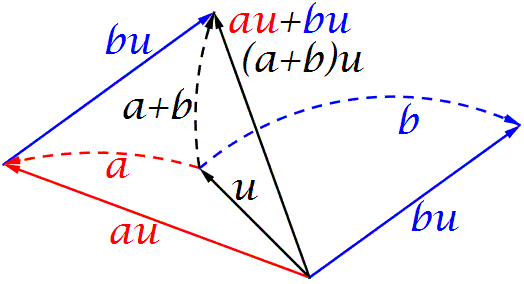
\includegraphics[width=0.5\textwidth]{imagenes/imagenes01/T01IM01.png}
		%\caption{Los dos problemas clásicos del cálculo: trazado de tangentes y áreas bajo curvas.}
	%\end{figure}
		
%varios párrafos encuadrados - explicaciones ad hoc
%\centering{
%\fbox{
%\parbox{0.95\textwidth}{
%varios
%
%$parrafos
%
%dentro
%}
%}
%}
% \justify


%\rotatebox{180}{\leftline{\textcolor{gris}{tararí}}}.